\documentclass[conference]{IEEEtran}
\IEEEoverridecommandlockouts

\usepackage{cite}
\usepackage{amsmath,amssymb,amsfonts}
\usepackage{algorithmic}
\usepackage{graphicx}
\usepackage{textcomp}
\usepackage{xcolor}

\usepackage{subcaption}

\def\BibTeX{{\rm B\kern-.05em{\sc i\kern-.025em b}\kern-.08em
    T\kern-.1667em\lower.7ex\hbox{E}\kern-.125emX}}

\begin{document}

	\title{On Existing Min Area Polygonalization Algorithms And Possible Improvements\\}
	
	\author{\IEEEauthorblockN{Maksym Kovalchuk}
	\IEEEauthorblockA{\textit{Faculty of Computer Sciences and Cybernetics} \\
	\textit{Taras Shevchenko national university of Kyiv}\\
	Kyiv, Ukraine \\
	max.koval4uk@ukr.net}
	}
	
	\maketitle
	
	\begin{abstract}
		It was proven that Minimum Area Polygonalization (MAP) problem belongs to the NP-Hard set of problems.
		Therefore, different approximation algorithms were developed.
		In this paper, we suggest a modification to the recently proposed application of the "Divide And Conquer" technique to the MAP problem.
		Our algorithm computes slightly more cases and often outperforms other algorithms in terms of polygon area.
		The complexity of the modified algorithm is $\bold{O(n^{2}log(n))}$ using $\bold{O(n)}$ memory.
		We also introduce postprocessing technique.
		It takes solutions from other algorithms and makes local points rearrangement if it minimizes polygon area.
		The complexity of postprocessing is $\bold{O(n^{2})}$ using $\bold{O(n)}$ memory.
		Experimental results indicate that it is expedient to use our algorithm in combination with postprocessing under time pressure.
		If no time pressure it is also useful to try randomized MAP algorithms in combination with postprocessing.
	\end{abstract}
	
	\begin{IEEEkeywords}
		computational geometry, minimum area polygonalization, divide and conquer, postprocessing
	\end{IEEEkeywords}
	
	
	\section{Introduction}
	\label{S1}
		Computational Geometry plays important role in nowadays problemsolving.
		It offers various solutions for both deeply theoretical research and applied software.
		One type of problem is constructing different shapes optimizing parameters like perimeter and area.
		
		In this paper, we consider the problem of finding the minimal area polygon (MAP), vertices of which are all points from the given set.
		In practice, this problem arises in the context of geo-sensor networks \cite{link1, link2}, and GIS systems \cite{link3, link4}.
		Like Traveling Salesman Problem, MAP is NP-hard, which was proven in \cite{link5}.
		It makes it almost impossible to solve the problem provably optimal for big enough data sets.
		Most related works focus on approximation of MAP, rather than finding the best possible polygonalization.
	
		The simplest algorithm for finding optimal MAP is MAP{\textunderscore}PermuteAndReject with complexity $O(n!)$.
		MAP{\textunderscore}PermuteAndReject brute-force all permutations, each corresponding unique polygon, checks if the polygon is simple and takes one with minimal area.
		In \cite{link9, link10} MAP was formulated as the IP problem. Such an approach works faster than MAP{\textunderscore}PermuteAndReject without losing optimality.
		MAP for 24 points was computed in about 90000 seconds \cite{link10}.
	
		Algorithm MAP{\textunderscore}Greedy proposed in \cite{link8}.
		The idea is to start with the convex hull of points and iteratively add feasible points that form maximal area triangle with edges of the previously computed polygon.
		The complexity of the algorithm is $O(n^{3})$ with $O(n^{2})$ memory usage.
		Algorithm MAP{\textunderscore}DAC with complexity $O(n^{2})$ described in \cite{link13}.
		Authors on each step divide point set on 2 subsets, recursively solve the
		problem for smaller sets and merge found polygons with minimal area quadrilateral.
		If the subset of the points has less than 6 elements MAP{\textunderscore}PermuteAndReject is used.
	
		Randomized algorithms were proposed in \cite{link11, link12}.
		MAP{\textunderscore}RS \cite{link12} consist of 6 strategies how to choose the initial triangle, next point, and next edge.
		We believe that complexity of MAP{\textunderscore}RS is $O(q n^{3})$, where q is the number of trials and n is the number of points.
		MAP{\textunderscore}RAND \cite{link11} starts with the triangle.
		On each step, it chooses a random point and connects it with the edge that minimizes the polygon area.
		MAP{\textunderscore}RAND is the only algorithm that processes both inside the polygon and outside the polygon types of points.
		In \cite{link11} MAP{\textunderscore}RAND described with $O(q n^{2}log(n))$ complexity, but we believe that complexity can be improved to $O(q n^{2})$ using linear time polygon visibility algorithm \cite{link14}.
		In \cite{link12} algorithm based on Ant Colony Optimization was proposed.
	
		The rest of this article is organized as follows.
		In section \ref{S2}, we formulate the MAP problem, describe a modification to the MAP{\textunderscore}DAC algorithm, and propose a simple postprocessing technique.
		In section \ref{S3}, we analyze the complexity of described algorithms and their correctness.
		In section \ref{S4}, we present implementation details, a comparison of MAP{\textunderscore}DAC2 with the existing approximation MAP algorithms, and results of postprocessing output of other algorithms.
		We present our conclusion in Section \ref{S5}.
	
	
	\section{Proposed Algorithms}
	\label{S2}
		\textbf{Problem MAP.}
		A set S of n points is given on a plane.
		It is necessary to construct a simple polygon with the smallest possible area, which would cover a given set of points, and which vertices are all points of the set S.
	
		\subsection{Modification of MAP{\textunderscore}DAC}
			Proposed in \cite{link13} algorithm performs next steps.
			\begin{enumerate}
				\item If the number of points is less than 6, return MAP using MAP{\textunderscore}PermuteAndReject;
				\item Sort out all given points by X coordinate;
				\item Split sorted points into 2 subsets $S_{1}$ and $S_{2}$;
				\item Solve recursively (from step 1) for $S_{1}$ and $S_{2}$, getting polygons $P_{1}$ and $P_{2}$;
				\item Find minimal area quadrilateral Q connecting $P_{1}$ and $P_{2}$;
				\item Merge $P_{1}$ and $P_{2}$ based on Q and return result.
			\end {enumerate}
			
			In such a way we always split the point set by the vertical line.
			We can consider lines with different slope, but while it can be optimal for some point subsets it would not for other.
			
			Therefore we propose to maintain 2 solutions for each point subset, one for vertical separation and other for horizontal separation.
			In such a way we bring more local optimality without much loss of execution time efficiency.
				
			Our algorithm MAP{\textunderscore}DAC2 performs the next steps.
			\begin{enumerate}
				\item If the number of points is less than 6, return MAP using MAP{\textunderscore}PermuteAndReject;
				\item Sort out all given points by X coordinate and split sorted points into 2 subsets $S_{x}^{1}$ and $S_{x}^{2}$;
				\item Solve recursively (from step 1) for $S_{x}^{1}$ and $S_{x}^{2}$ getting polygons $P_{x}^{1,1}$, $P_{x}^{1,2}$, $P_{x}^{2,1}$ and $P_{x}^{2,2}$;
				\item Consider polygons $PM_{x}^{1}$, $PM_{x}^{2}$, $PM_{x}^{3}$, $PM_{x}^{4}$ received by merging pairs 
				\{$P_{x}^{1,1}$, $P_{x}^{2,1}$\}, 
				\{$P_{x}^{1,1}$, $P_{x}^{2,2}$\}, 
				\{$P_{x}^{1,2}$, $P_{x}^{2,1}$\}, 
				\{$P_{x}^{1,2}$, $P_{x}^{2,2}$\} respectively;
				\item  Let $P_{x}$ be one of the $PM_{x}^{1}$, $PM_{x}^{2}$, $PM_{x}^{3}$, $PM_{x}^{4}$ with the minimal area;
				\item Sort out all given points by Y coordinate and split sorted points into 2 subsets $S_{y}^{1}$ and $S_{y}^{2}$;
				\item Solve recursively (from step 1) for $S_{y}^{1}$ and $S_{y}^{2}$ getting polygons $P_{y}^{1,1}$, $P_{y}^{1,2}$, $P_{y}^{2,1}$ and $P_{y}^{2,2}$;
				\item Consider polygons $PM_{y}^{1}$, $PM_{y}^{2}$, $PM_{y}^{3}$, $PM_{y}^{4}$ received by merging pairs 
				\{$P_{y}^{1,1}$, $P_{y}^{2,1}$\}, 
				\{$P_{y}^{1,1}$, $P_{y}^{2,2}$\}, 
				\{$P_{y}^{1,2}$, $P_{y}^{2,1}$\}, 
				\{$P_{y}^{1,2}$, $P_{y}^{2,2}$\} respectively;
				\item Let $P_{y}$ be one of the $PM_{y}^{1}$, $PM_{y}^{2}$, $PM_{y}^{3}$, $PM_{y}^{4}$ with the minimal area;
				\item Return pair \{$P_{x}$, $P_{y}$\}.
			\end {enumerate}
			
			All steps of MAP{\textunderscore}DAC2 except 4 and 8 are straightforward.
			Step 4 is described in the original paper for MAP{\textunderscore}DAC \cite{link13} and can be done in the next way.
			\begin{enumerate}
				\item Build polygon $E$ enclosing area between polygons $A$ and $B$.
				It consists of 2 chains, 1 from each of given polygons, and 2 tangents that connect border points of chains;
				\item For all points of the first chain find all visible points on the second chain \cite{link14};
				\item For all consecutive point pairs of the first chain find all visible consecutive point pairs on the second chain that form simple quadrilateral.
				Choose the smallest quadrilateral. 
			\end {enumerate}
			Step 8 is almost the same as 4, but with horizontal separation.
			In case implementation is hardcoded for vertical separation, it is possible to interchange X and Y coordinates of points to bring step 8 to 4.
			8 polygons considered on steps 4 and 8 are shown in Fig. \ref{fig1}.
			
			\begin{figure}[htbp]
				\centering
				\begin{subfigure}{0.45\linewidth}
					\centering
					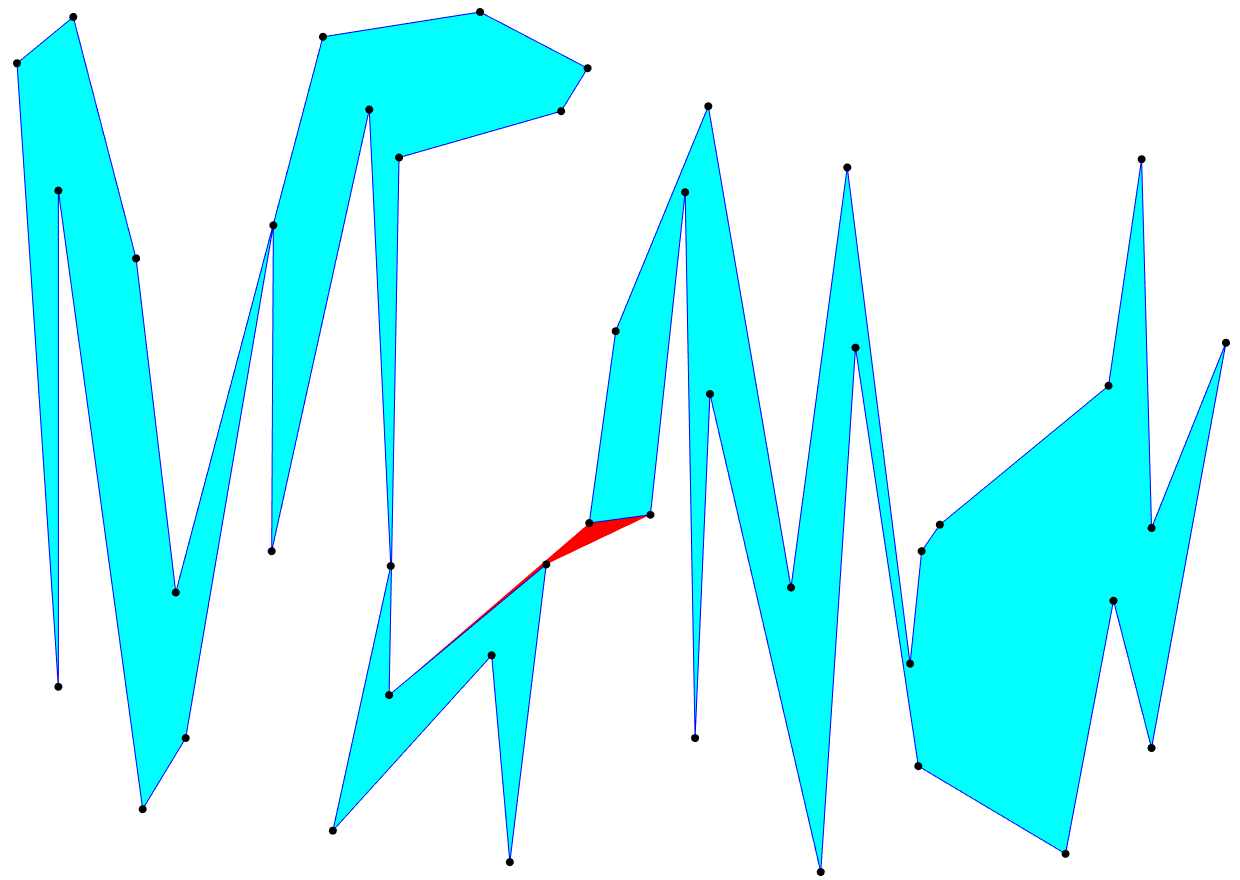
\includegraphics[width=0.99\textwidth]{fig1a.png}
					\caption{}
					\label{fig1a}
				\end{subfigure}
				\begin{subfigure}{0.45\linewidth}
					\centering
					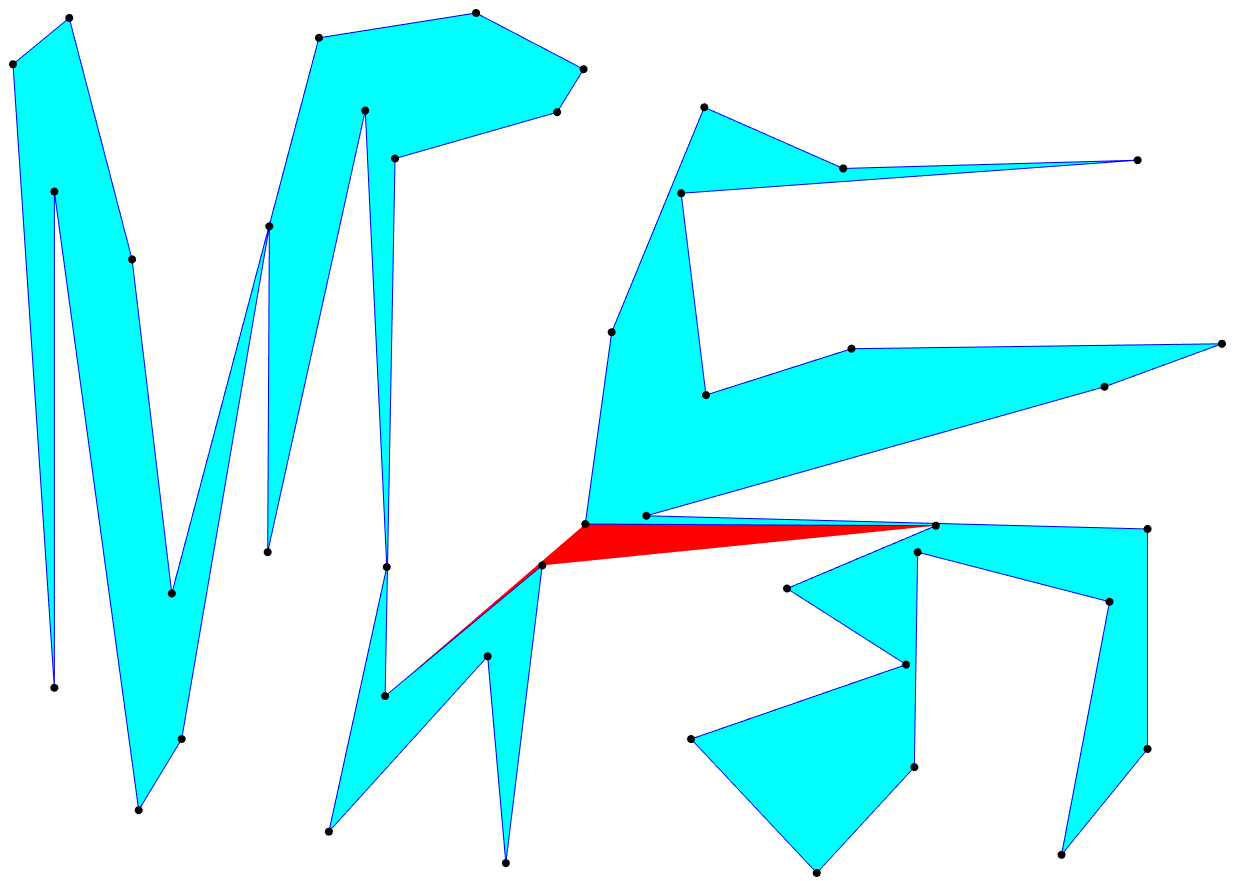
\includegraphics[width=0.99\textwidth]{fig1b.png}
					\caption{}
					\label{fig1b}
				\end{subfigure}
				
				\begin{subfigure}{0.45\linewidth}
					\centering
					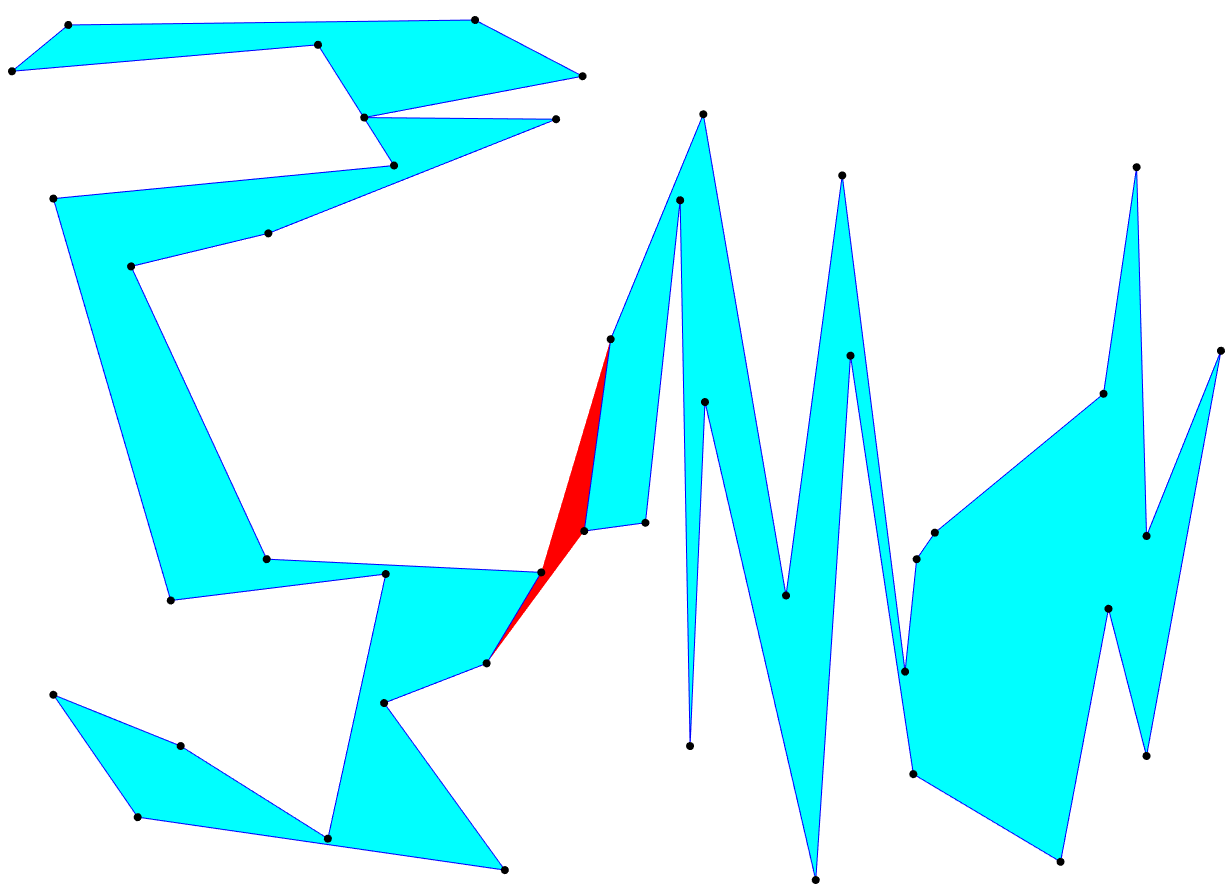
\includegraphics[width=0.99\textwidth]{fig1c.png}
					\caption{}
					\label{fig1c}
				\end{subfigure}
				\begin{subfigure}{0.45\linewidth}
					\centering
					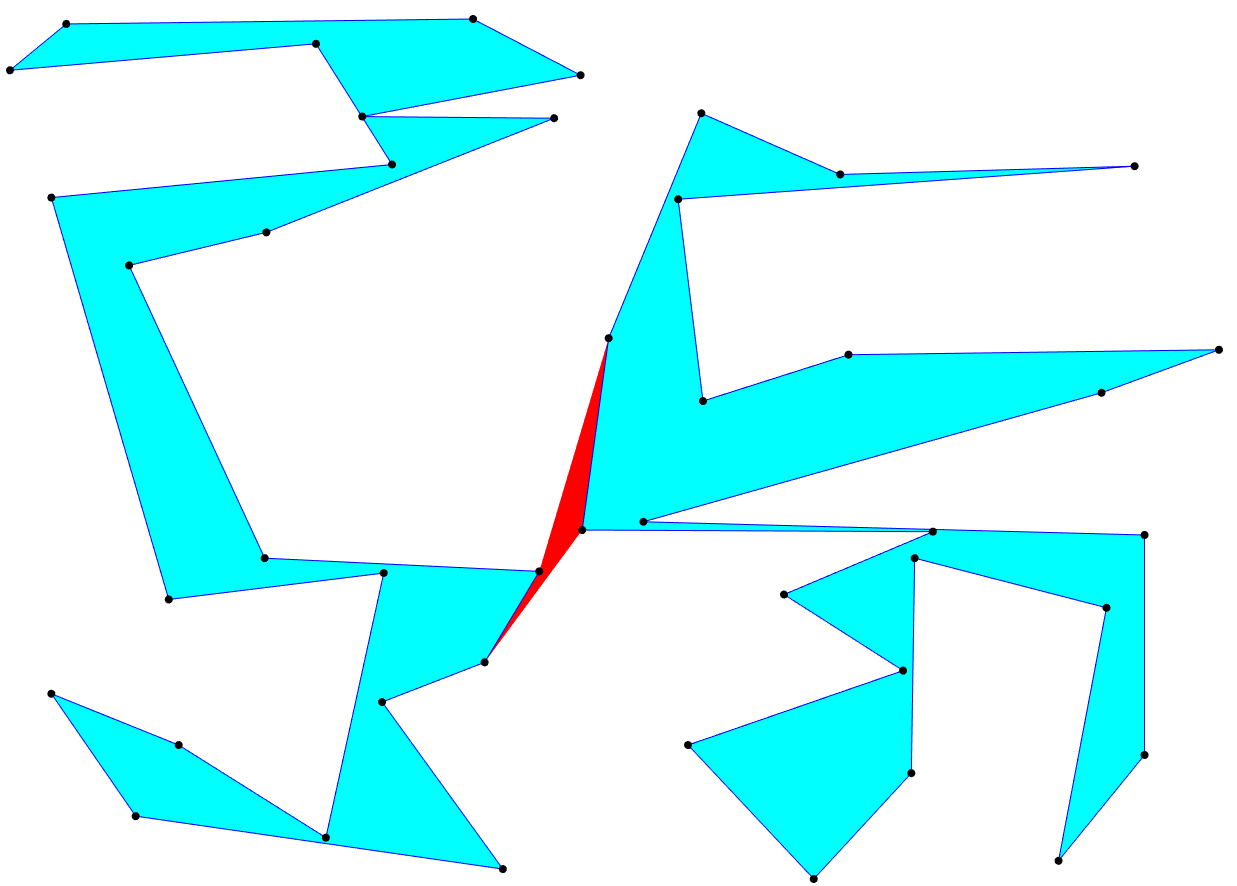
\includegraphics[width=0.99\textwidth]{fig1d.png}
					\caption{}
					\label{fig1d}
				\end{subfigure}
				
				\begin{subfigure}{0.45\linewidth}
					\centering
					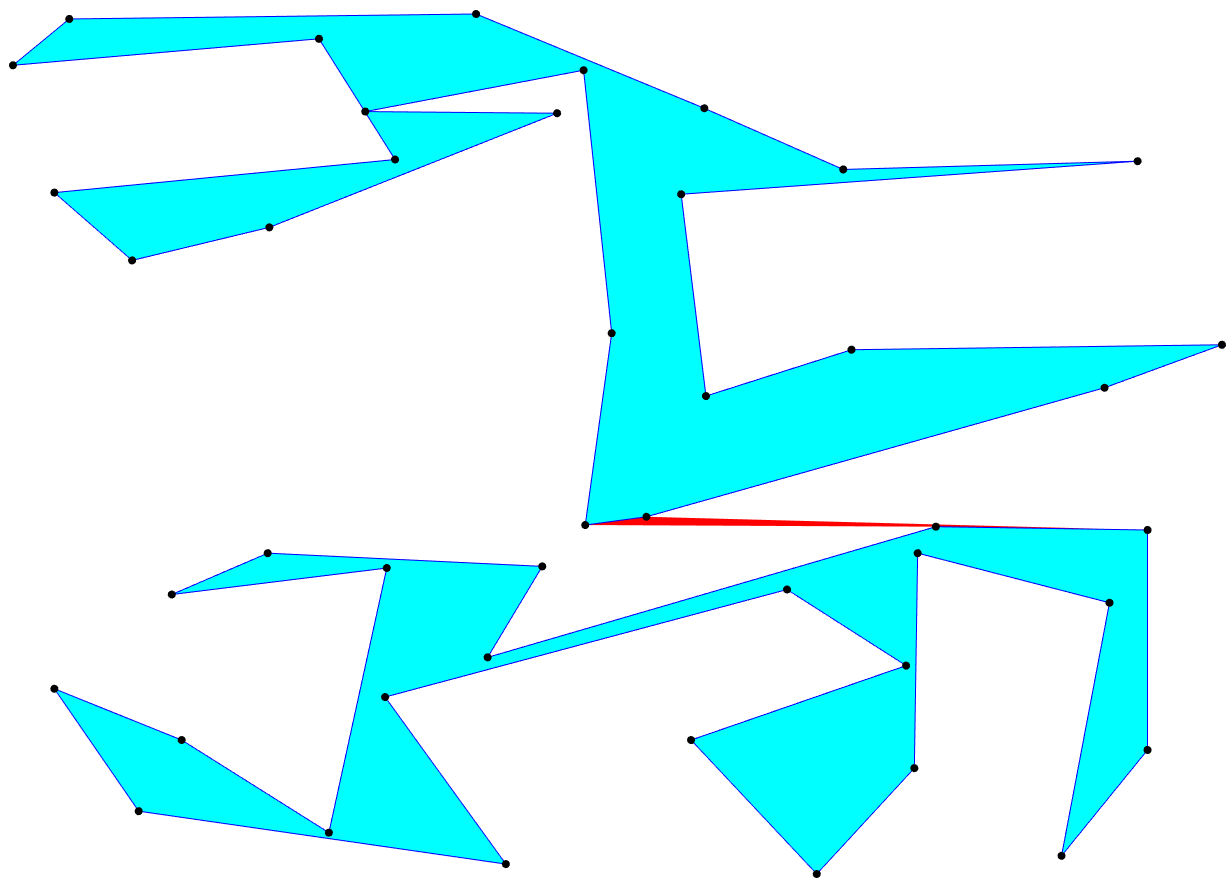
\includegraphics[width=0.99\textwidth]{fig1e.png}
					\caption{}
					\label{fig1e}
				\end{subfigure}
				\begin{subfigure}{0.45\linewidth}
					\centering
					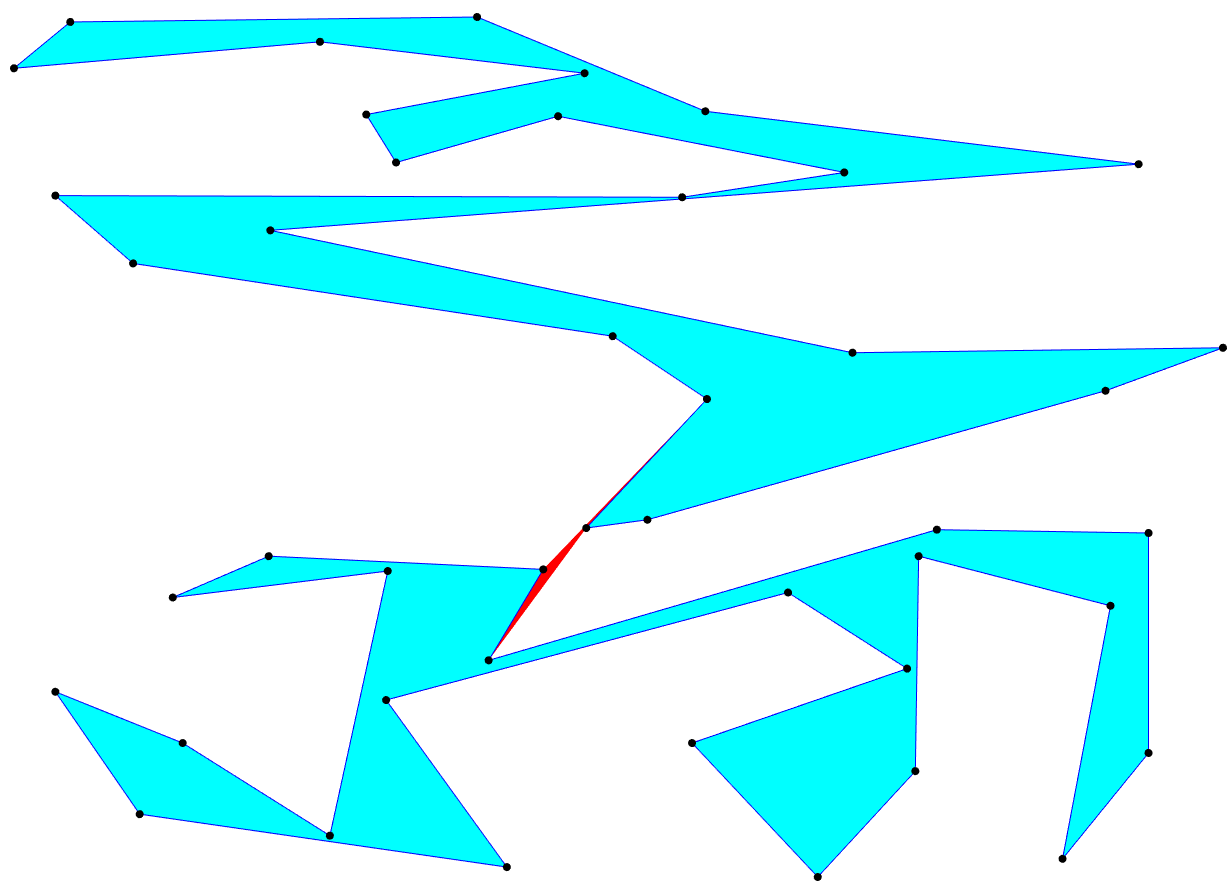
\includegraphics[width=0.99\textwidth]{fig1f.png}
					\caption{}
					\label{fig1f}
				\end{subfigure}
				
				\begin{subfigure}{0.45\linewidth}
					\centering
					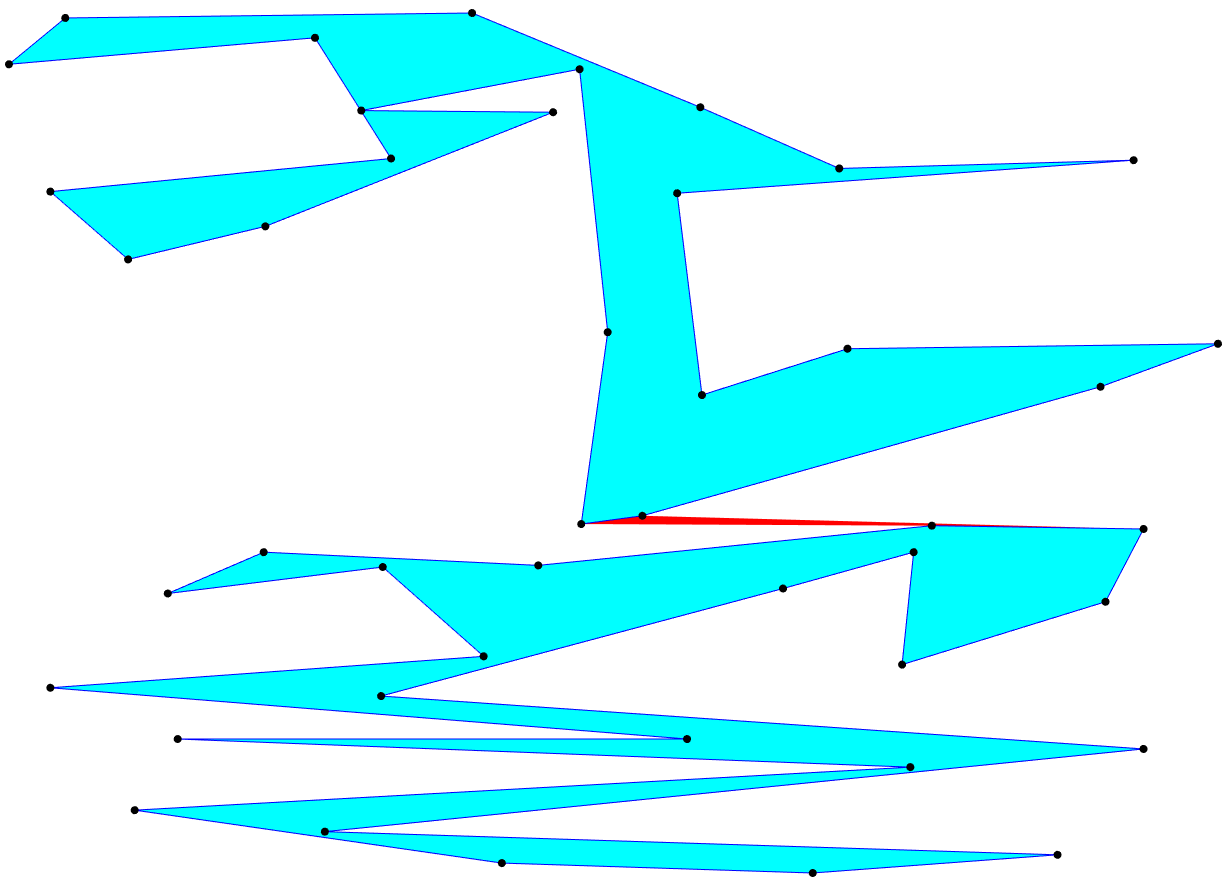
\includegraphics[width=0.99\textwidth]{fig1g.png}
					\caption{}
					\label{fig1g}
				\end{subfigure}
				\begin{subfigure}{0.45\linewidth}
					\centering
					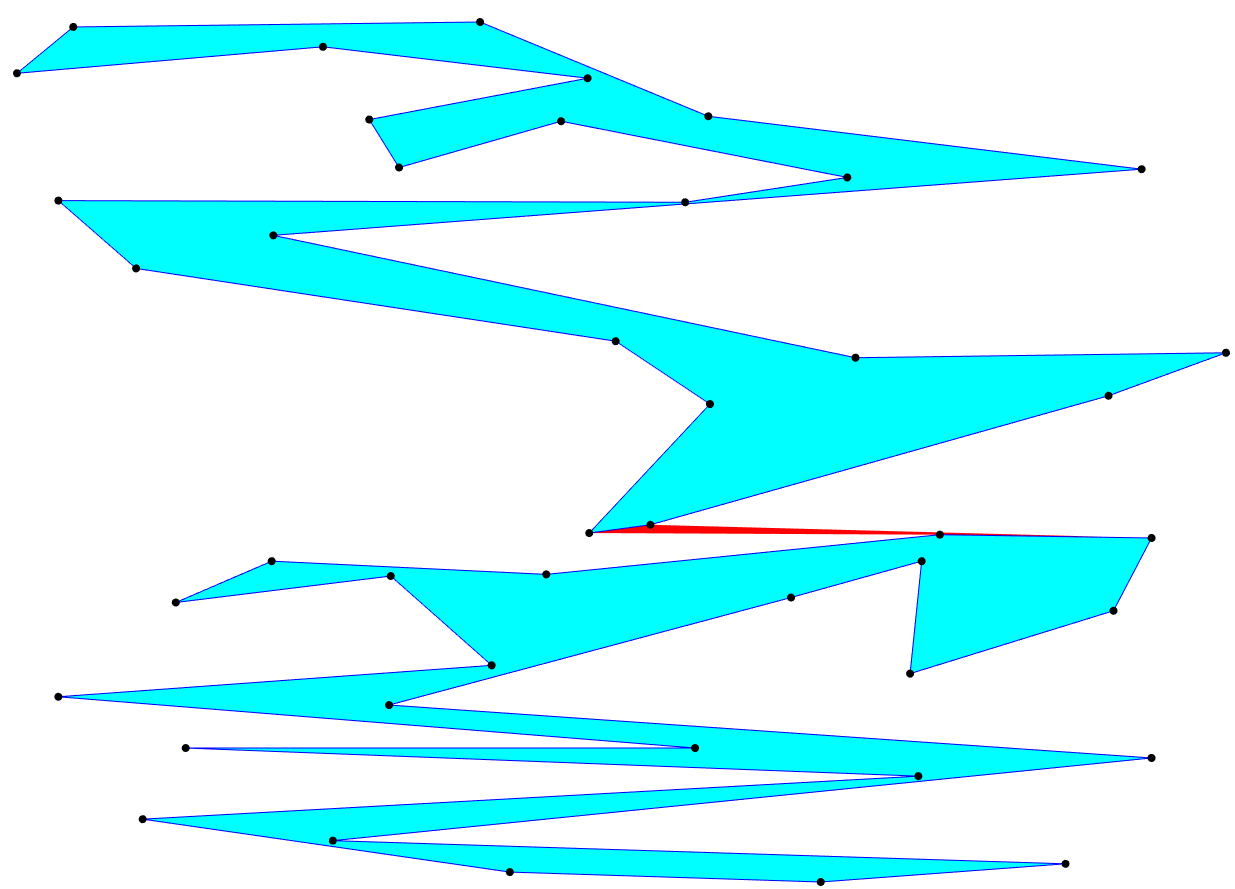
\includegraphics[width=0.99\textwidth]{fig1h.png}
					\caption{}
					\label{fig1h}
				\end{subfigure}
				
				\caption
				{
					8 different polygons considered in MAP{\textunderscore}DAC2 (blue -- polygons recieved recursively, red -- merging quadrilateral).
					(a) $PM_{x}^{1}$
					(b) $PM_{x}^{2}$
					(c) $PM_{x}^{3}$
					(d) $PM_{x}^{4}$
					(e) $PM_{y}^{1}$
					(f) $PM_{y}^{2}$
					(g) $PM_{y}^{3}$
					(h) $PM_{y}^{4}$
				}
				\label{fig1}
			\end{figure}
		
		\subsection{Postprocessing of MAP solution}
			It is typical for MAP approximation algorithms to use heuristics that greedily choose point, edge, quadrilateral, etc.
			Such heuristics may be optimal on the current step but can be nonoptimal in the future.
			We propose a simple postprocessing technique that removes 1 point at a time and tries to add it in the more optimal position.
			Postprocessing lies in the next steps.
			\begin{enumerate}
				\item Consider all points $P_{i}$ of polygon $P = P_{1}, P_{2}, ..., P_{n}$ one by one;
				\item If we can remove $P_{i}$ such that $P^{*} = P_{1}, ..., P_{i-1}, P_{i+1}, ..., P_{n}$ is simple polygon (*) 
				and segment $(P_{i-1}, P_{i+1})$ of $P^{*}$ is visible from $P_{i}$ (**) 
				then remove $P_{i}$ else goto step 1 and consider next point;
				\item If $P_{i}$ is inside $P^{*}$ then find edge $(P_{j-1}, P_{j})$ of $P^{*}$ visible from $P_{i}$ that maximize area of triangle \{$(P_{j-1}, P_{i}, P_{j})$\}. 
				If $P_{i}$ is outside  $P^{*}$ then find edge $(P_{j-1}, P_{j})$ of $P^{*}$ visible from $P_{i}$ that minimize area of triangle \{$(P_{j-1}, P_{i}, P_{j})$\};
				\item Insert $P_{i}$ such that new value of polygon $P = P_{1}, ..., P_{j-1}, P_{i}, P_{j}, ..., P_{n}$ and goto step 1 considering next point.
			\end{enumerate}
			
			To check (*) we can simply check whether edge $(P_{i-1}, P_{i+1})$ intersect other edges of $P^{*}$.
			To check (**) we can use the visibility polygon algorithm proposed in \cite{link14}.
			To check whether 4 a point is inside or outside of the polygon we can use the windmill algorithm.
			To find edge $(P_{j-1}, P_{j})$ we can use visibility polygon computed when checking (**).
			
			In practice, we ran several trials of postprocessing until no more area minimizing points rearrangements are possible.
			Example of postprocessing optimization is shown in Fig. \ref{fig2}.
			
			\begin{figure}[htbp]
				\centering
				\begin{subfigure}{0.32\linewidth}
					\centering
					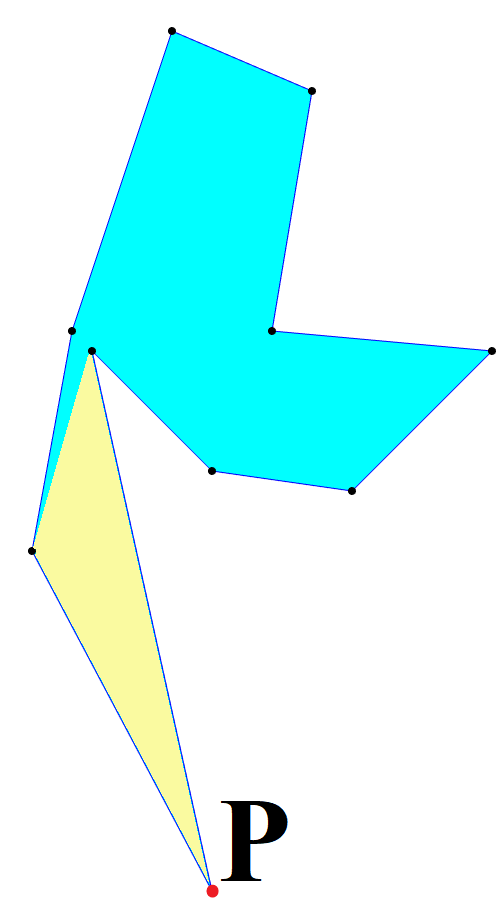
\includegraphics[width=0.99\textwidth]{fig2a.png}
					\caption{}
					\label{fig2a}
				\end{subfigure}
				\begin{subfigure}{0.32\linewidth}
					\centering
					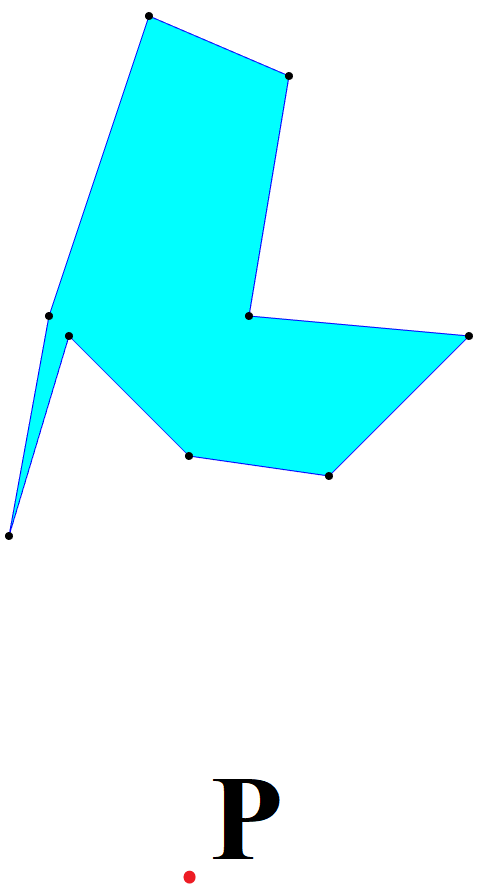
\includegraphics[width=0.99\textwidth]{fig2b.png}
					\caption{}
					\label{fig2b}
				\end{subfigure}
				\begin{subfigure}{0.32\linewidth}
					\centering
					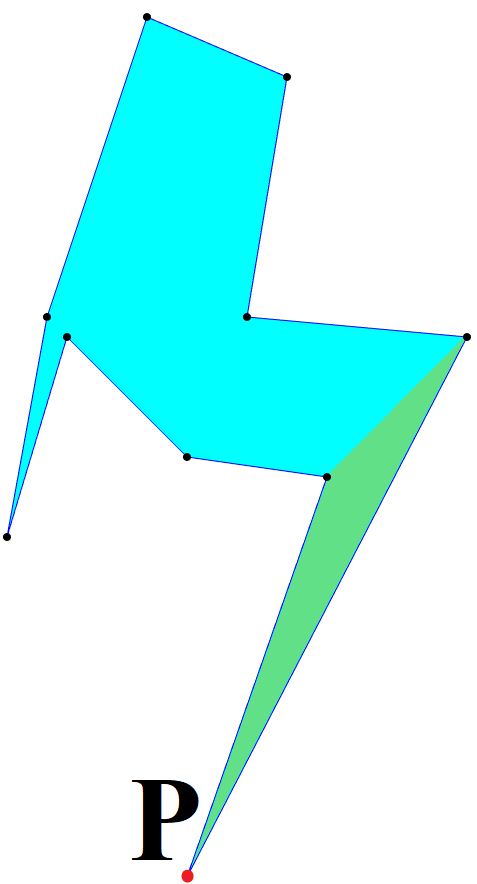
\includegraphics[width=0.99\textwidth]{fig2c.png}
					\caption{}
					\label{fig2c}
				\end{subfigure}
				
				\caption
				{
					Example of postprocessing (red point $P$ is postprocessed, yellow -- removed triangle, green -- added triangle).
					(a) initial polygon
					(b) $P$ removed from polygon
					(c) $P$ inserted in better position
				}
				\label{fig2}
			\end{figure}
	
	\section {Complexity and Correctness}
	\label{S3}
		\subsection {Complexity}
			\textbf{Theorem 1.}
			Algorithm MAP{\textunderscore}DAC2 can be implemented with complexity $O(n^{2}log(n))$.
			
			\textit{Proof.}
			MAP{\textunderscore}DAC2 is recursive algorithm.
			During the one iteration, it sorts out points twice, calls merging function 8 times, and calls itself recursively 4 times with 2 times smaller point set.
			Complexity of sorting is $O(n log(n))$.
			Complexity of merging function is $O(n^{2})$ [13].
			That is we have recurrence $T(n) = 4*T(n/2) + 8 * O(n^{2}) + 2 * O(n log(n))$.
			After simplification we get $T(n) = 4*T(n/2) + O(n^{2})$.
			Last recurrence can be solved using Master Theorem and the solution is $O(n^{2}log(n))$.
	
			\textbf{Theorem 2.}
			Postprocessing can be implemented with complexity $O(n^{2})$.
			
			\textit{Proof.}
			We can check (*) and (**) as described above in $O(n)$ time.
			The complexity of the windmill algorithm is also $O(n)$.
			If while checking (**) visibility polygon already constructed then we can find edge $(P_{j-1}, P_{j})$ of step 4 with complexity $O(n)$.
			Therefore, we can process one point in $O(n)$ time.
			We need to process n points which lead to overall complexity $O(n^{2})$.
	
			In practice, we ran postprocessing several times until the polygon area converge.
			During the experimental study, maximal number of postprocessing trials was 10.
			We believe that running postprocessing until area converges also has $O(n^{2})$ complexity.
			
		\subsection {Correctness of MAP{\textunderscore}DAC2}
			Correctness of MAP{\textunderscore}DAC2 consists in the existence of quadrilateral merging 2 polygons on steps 4 and 9.
			MAP{\textunderscore}DAC2 tries to merge 4 pairs of polygons on both step 4 and step 9.
			During the experimental study, we found pairs that cannot be merged as such a quadrilateral do not exist.
			Despite it, at least one of 4 pairs always could be combined when running MAP{\textunderscore}DAC2 on our data set.
			We don`t know whether it holds in the general case.
			In the implementation we assign infinity area to the incorrect polygonalization, leading the algorithm to choose one with a smaller area.
			In case the algorithm approved to be incorrect in general we suggest running several trials with randomly rotated input points.
	
		\subsection {Correctness of postprocessing}
			Trap region of polygon P is the area of the plane from which no edges of P are completely visible (Fig. \ref{fig3}).
			Concept of trap region introduced in \cite{link11}.
			Therefore, for the algorithm to be correct it is necessary to not lead input points into the trap region or somehow deal with the trap region otherwise.
			[11] propose to ran MAP{\textunderscore}RAND with different random seed in case of some point in the trap region.
			The same can be done in MAP{\textunderscore}RS.
			So, we can consider randomized algorithms to be correct.
			During the experimental study, MAP{\textunderscore}Greedy fell into the trap region several times.
			Because MAP{\textunderscore}Greedy described in \cite{link8} is a deterministic algorithm, we claim it to be incorrect in the general case.
			
			\begin{figure}[htbp]
				\centering
				\begin{subfigure}{0.49\linewidth}
					\centering
					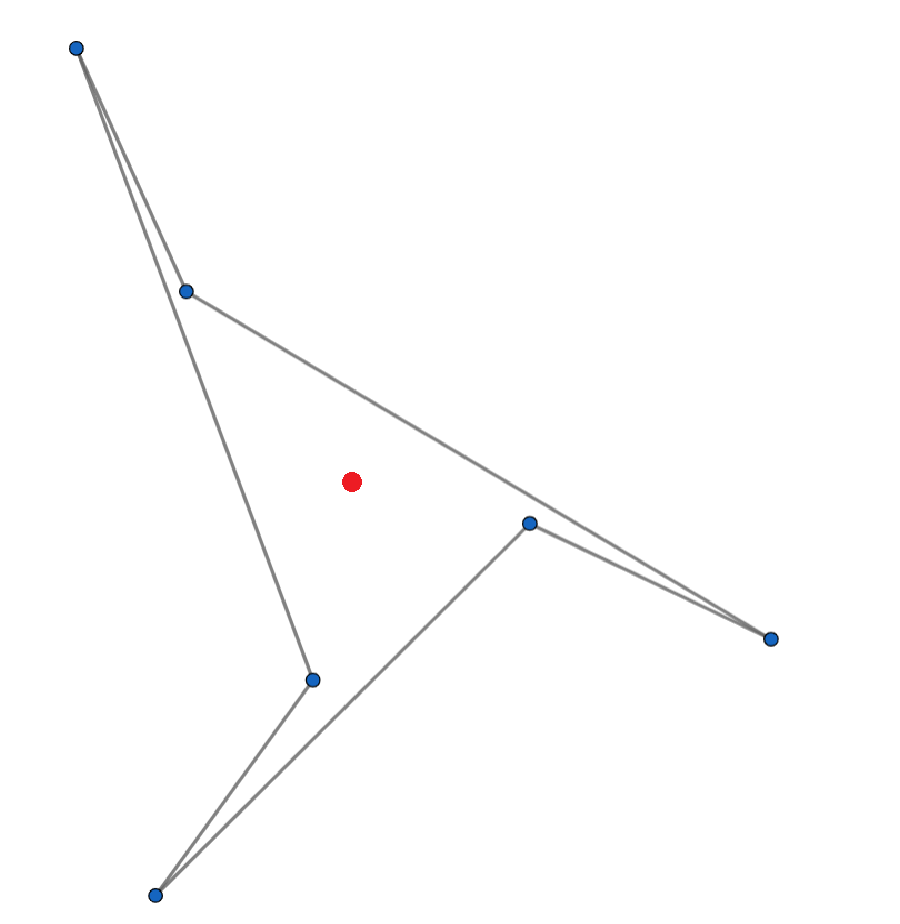
\includegraphics[width=0.99\textwidth]{fig3a.png}
					\caption{}
					\label{fig3a}
				\end{subfigure}
				\begin{subfigure}{0.49\linewidth}
					\centering
					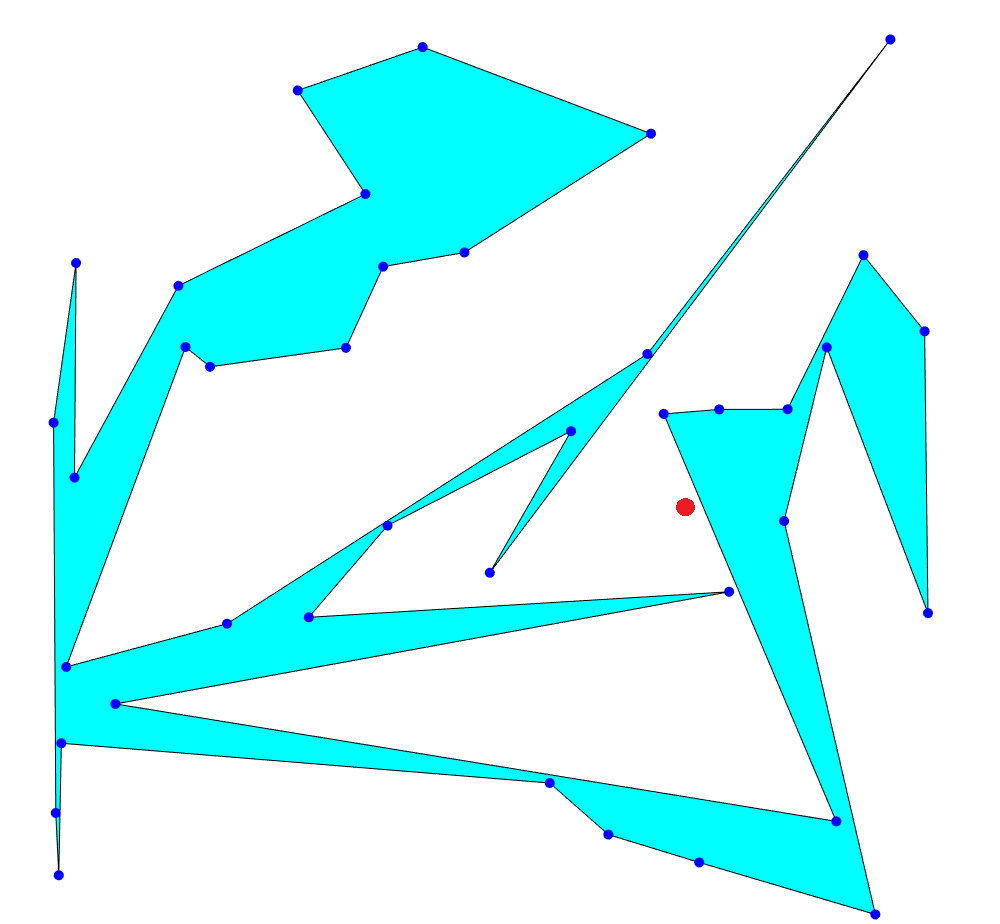
\includegraphics[width=0.99\textwidth]{fig3b.png}
					\caption{}
					\label{fig3b}
				\end{subfigure}
				\caption
				{
					Red point is inside the trap region.
					(a) point inside the polygon
					(b) point outside the polygon 
				}
				\label{fig3}
			\end{figure}

			\begin{figure*}[htbp]
				\centerline{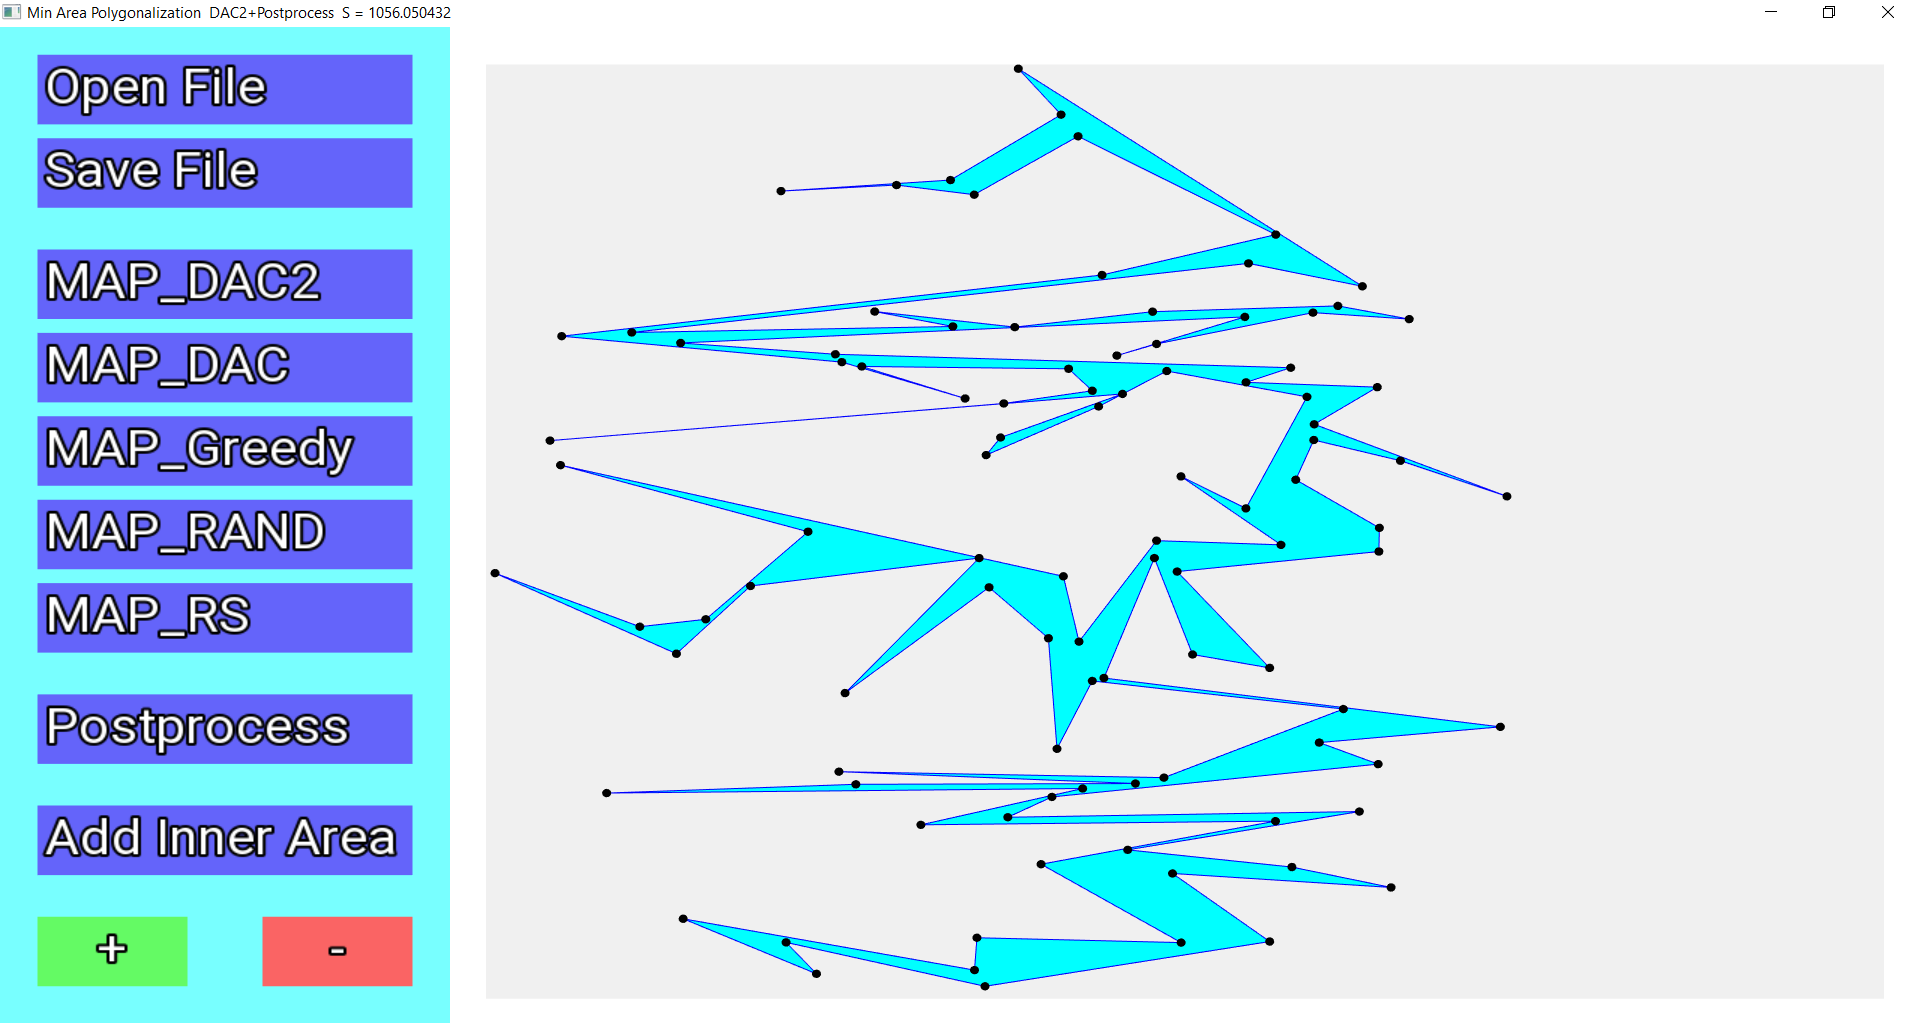
\includegraphics[width=0.9\textwidth]{fig4.png}}
				\caption{The interface of the developed program.}
				\label{fig4}
			\end{figure*}

			\textbf{Theorem 3.}
			The postprocessing algorithm never throws removed points into the trap region of $P^{*}$.
			The postprocessing algorithm either improves the area of the given polygon or does not change it.
			
			\textit{Proof.}
			For every point there possible 3 distinct cases.
			\begin{enumerate}
				\item (+) At least one of (*) or (**) does not hold and the point is not removed;
				\item (++) Point is removed and added such that old and new values of P are the same;
				\item (+++) Point is removed and added such that old and new values of P are not the same.
			\end{enumerate}
			
			In case (+), we do not remove points, therefore correctness is held.
			Otherwise (cases (++), (+++)) point is removed.
			In case (+++) not only correctness is held but also area is improved.
			If both (+) and (+++) are not met then from (+) we have guarantee of (**).
			That is, edge $(P_{i-1}, P_{i+1})$ of $P^{*}$ is visible from $(P_{i}$.
			So, removed point $P_{i}$ is not in the trap region but overall area remains the same as before (case (++)).
			
	\section{Experimental Results}
	\label{S4}
		To test described algorithms and compare them with previously proposed algorithms we have implemented MAP{\textunderscore}DAC2, MAP{\textunderscore}DAC, MAP{\textunderscore}Greedy, MAP{\textunderscore}RAND, MAP{\textunderscore}RS, and postprocessing.
		We write in C++ using the SFML library for a graphical interface (Fig. \ref{fig4}).
		There are 2 ways of specifying the data – reading points from the file and adding or deleting points via clicking on the drawing panel.
		
		To compare different algorithms 30 random point sets are generated.
		There are 3 types of point sets, each type consist of 10 sets of different sizes.
		The First 2 types are random points in rectangle and circle, named *{\textunderscore}square.txt and *{\textunderscore}circle.txt respectively.
		Points from the third type form a grid with some random shift from the exact position, named *{\textunderscore}grid.txt.
		Different types are shown in Fig. \ref{fig5}.
		
		\begin{figure}[htbp]
			\centering
			\begin{subfigure}{0.32\linewidth}
				\centering
				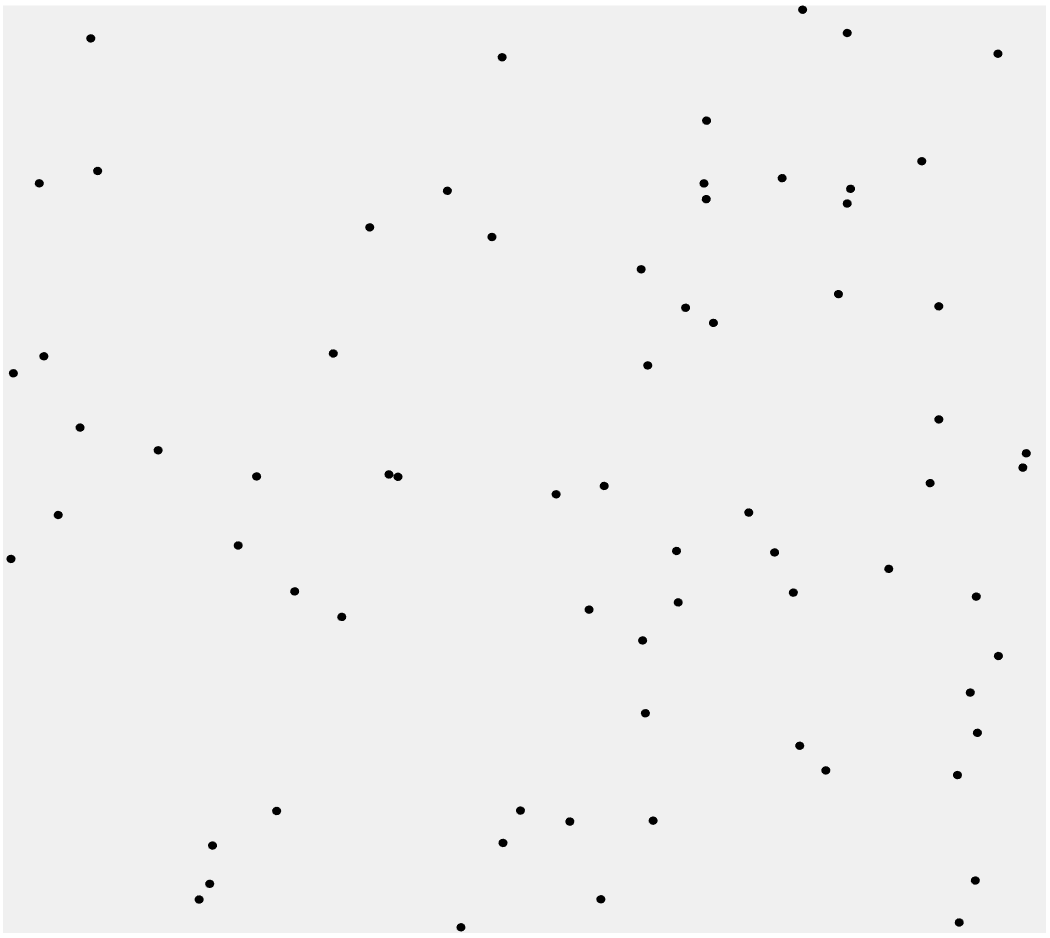
\includegraphics[width=0.99\textwidth]{fig5a.png}
				\caption{}
				\label{fig5a}
			\end{subfigure}
			\begin{subfigure}{0.32\linewidth}
				\centering
				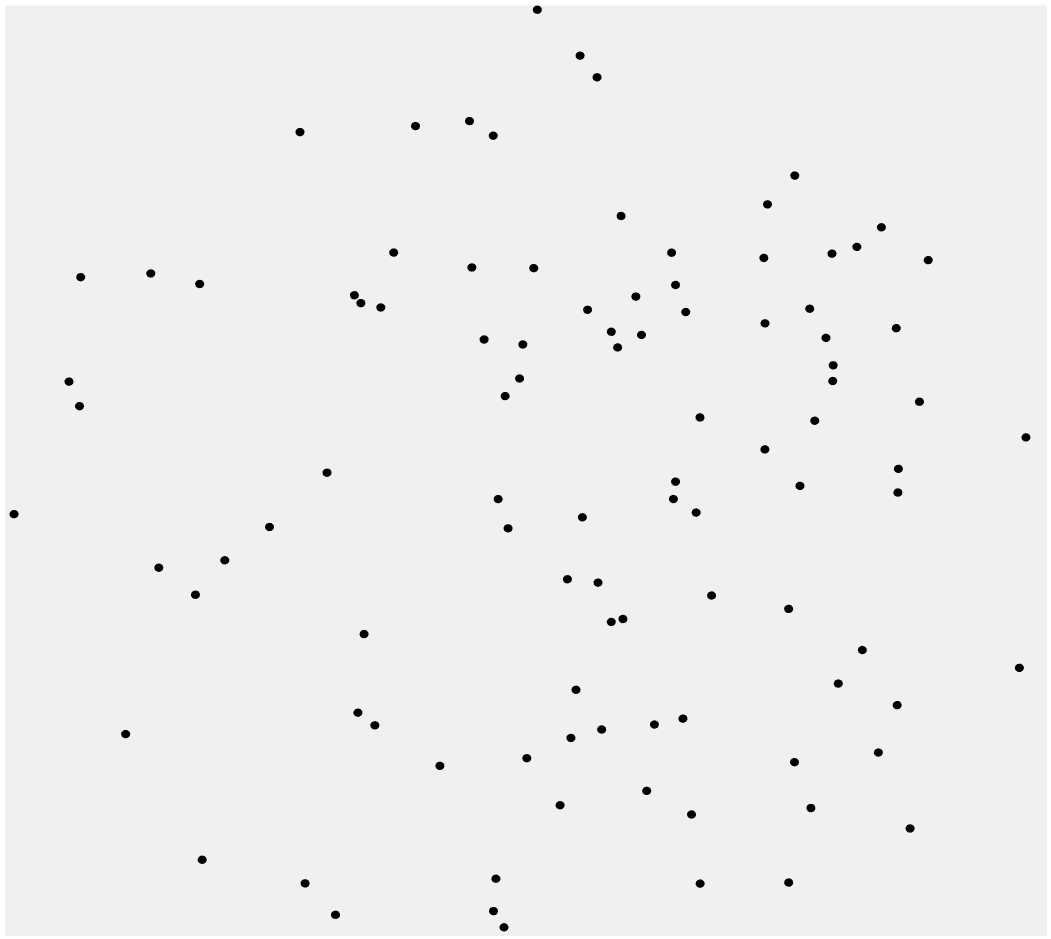
\includegraphics[width=0.99\textwidth]{fig5b.png}
				\caption{}
				\label{fig5b}
			\end{subfigure}
			\begin{subfigure}{0.32\linewidth}
				\centering
				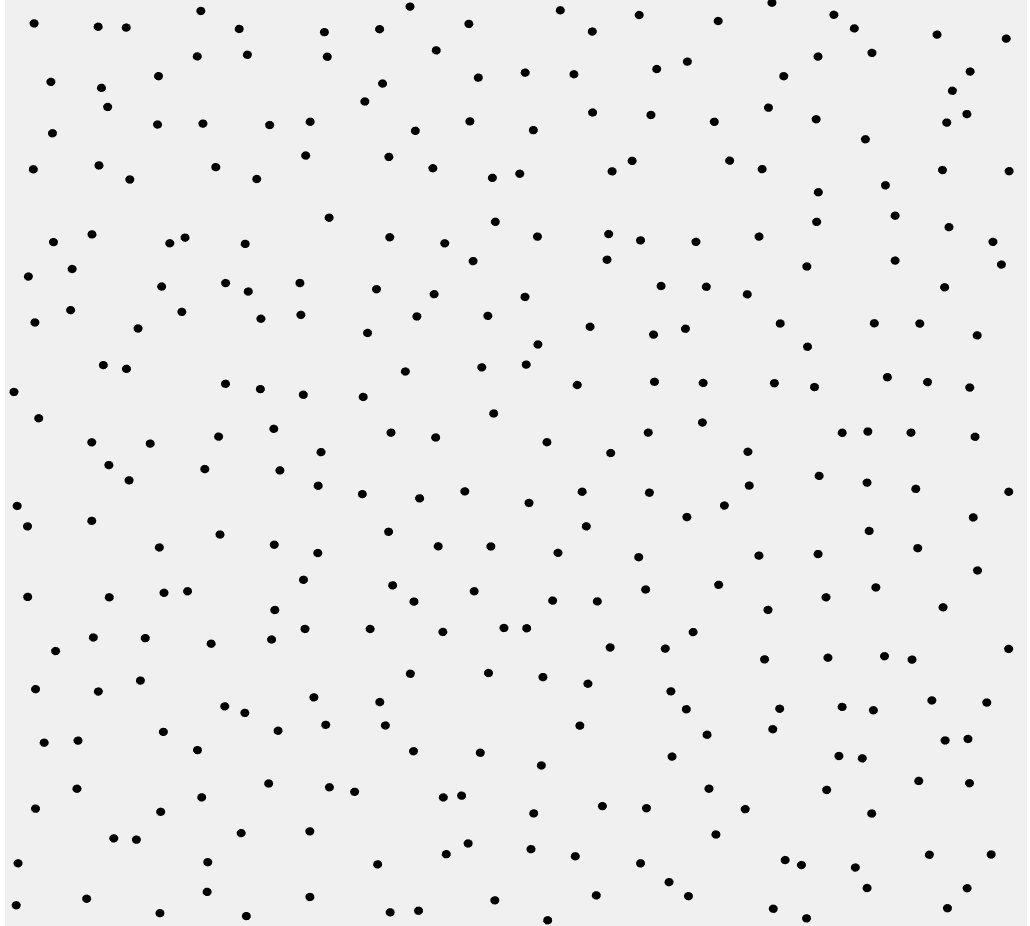
\includegraphics[width=0.99\textwidth]{fig5c.png}
				\caption{}
				\label{fig5c}
			\end{subfigure}
			\caption
			{
				(a) 1{\textunderscore}square.txt
				(b) 1{\textunderscore}circle.txt
				(c) 1{\textunderscore}grid.txt
			}
			\label{fig5}
		\end{figure}
	
		We ran all 5 algorithms on described point sets (Fig. \ref{fig6} (a)-(e)).
		For randomized algorithms MAP{\textunderscore}RAND and MAP{\textunderscore}RS we set $q=200$ trials and take the best produced polygonalization.
		Table \ref{table1} shows the results.
		As MAP{\textunderscore}Greedy was discovered to be incorrect, our implementation of this algorithm ignores points that are in the trap region.
		Cases with incorrect output polygonalization are noted with the asterisk.
		In 17 out of 30 cases the best result was computed by MAP{\textunderscore}DAC2.
		In the other 13 cases, the best polygonalization was computed by MAP{\textunderscore}RS.
		Regardless of MAP{\textunderscore}RS can outperform MAP{\textunderscore}DAC2 in terms of polygon area, MAP{\textunderscore}RS is quite slow relative to MAP{\textunderscore}DAC2 as their complexities are $O(q n^{3})$ and $O(n^{2}log(n))$ respectively.
		
		\begin{figure}[htbp]
			\centering
			\begin{subfigure}{0.85\linewidth}
				\centering
				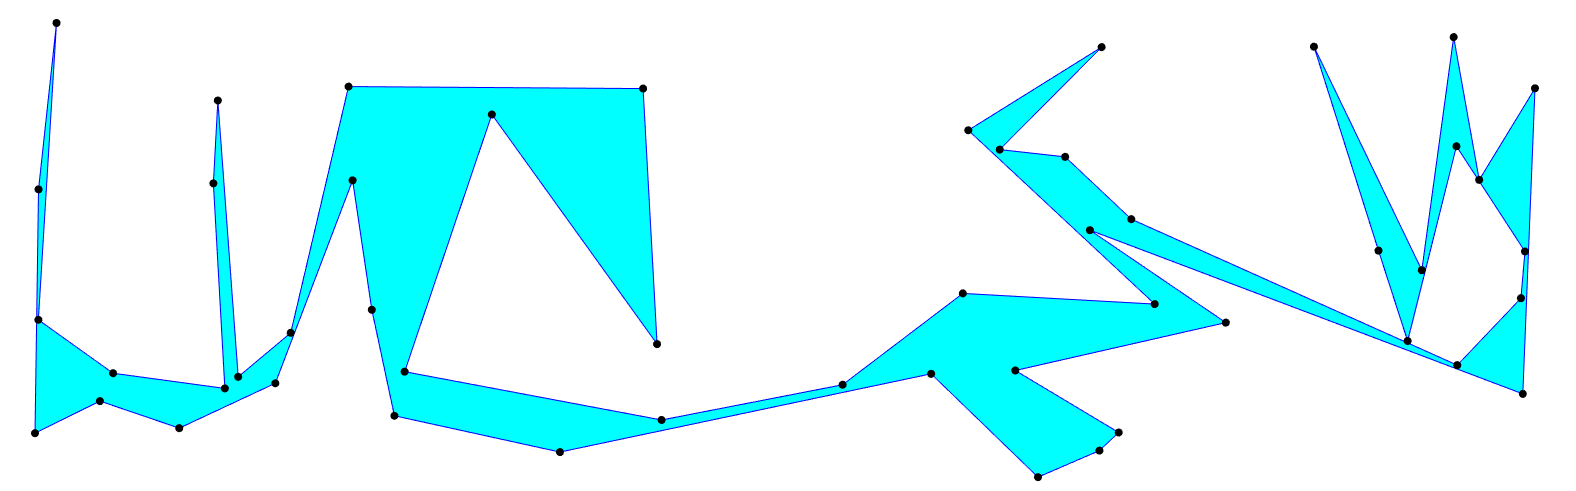
\includegraphics[width=0.99\textwidth]{fig6a.png}
				\caption{}
				\label{fig6a}
			\end{subfigure}
			
			\begin{subfigure}{0.85\linewidth}
				\centering
				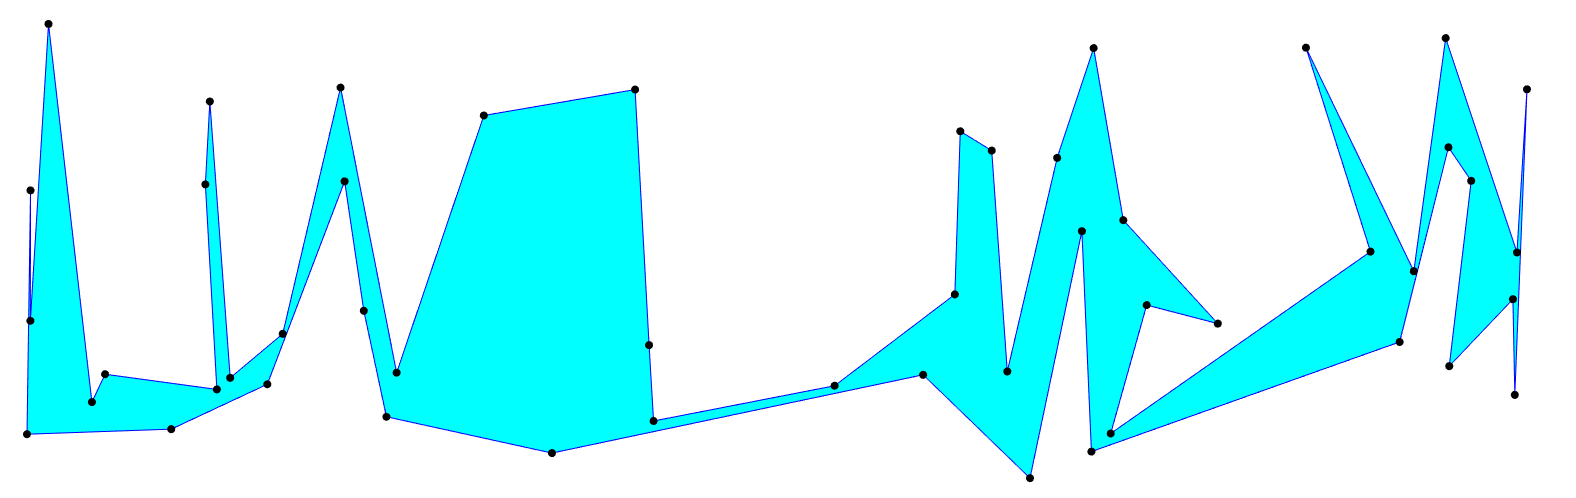
\includegraphics[width=0.99\textwidth]{fig6b.png}
				\caption{}
				\label{fig6b}
			\end{subfigure}
			
			\begin{subfigure}{0.85\linewidth}
				\centering
				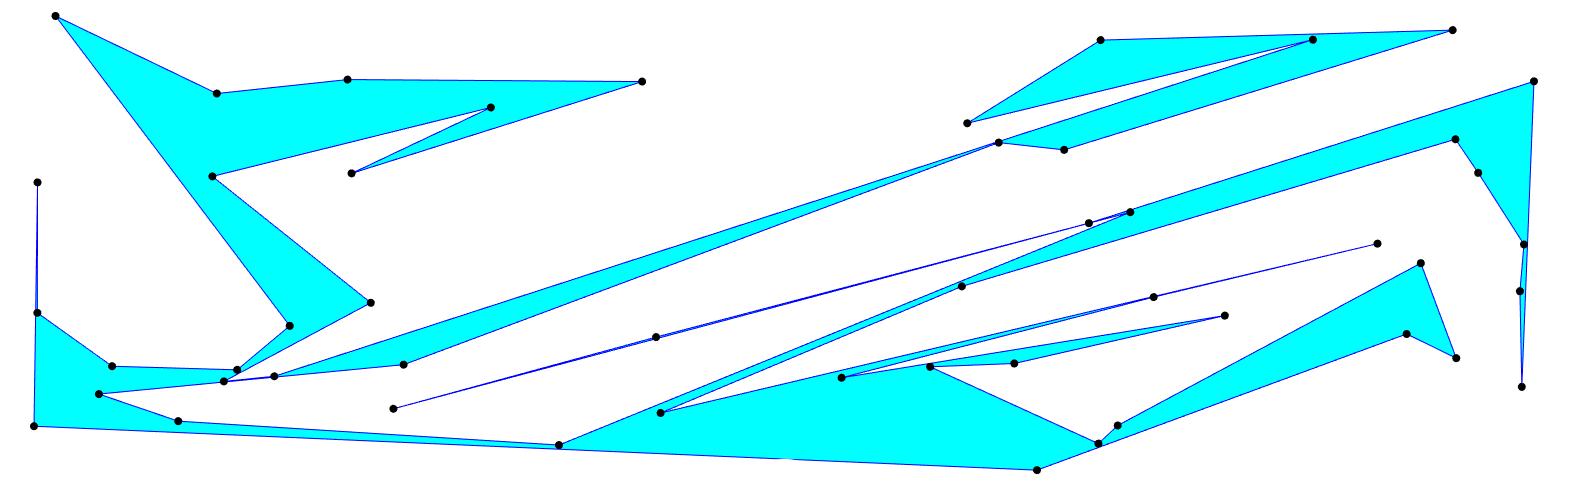
\includegraphics[width=0.99\textwidth]{fig6c.png}
				\caption{}
				\label{fig6c}
			\end{subfigure}
			
			\begin{subfigure}{0.85\linewidth}
				\centering
				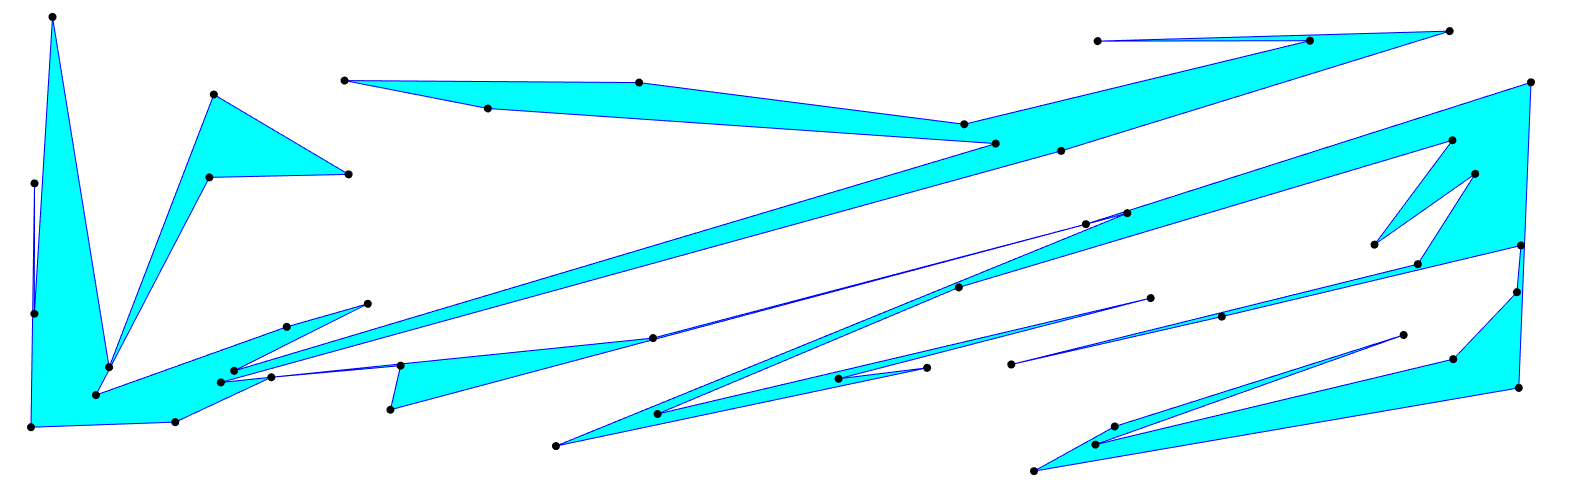
\includegraphics[width=0.99\textwidth]{fig6d.png}
				\caption{}
				\label{fig6d}
			\end{subfigure}
			
			\begin{subfigure}{0.85\linewidth}
				\centering
				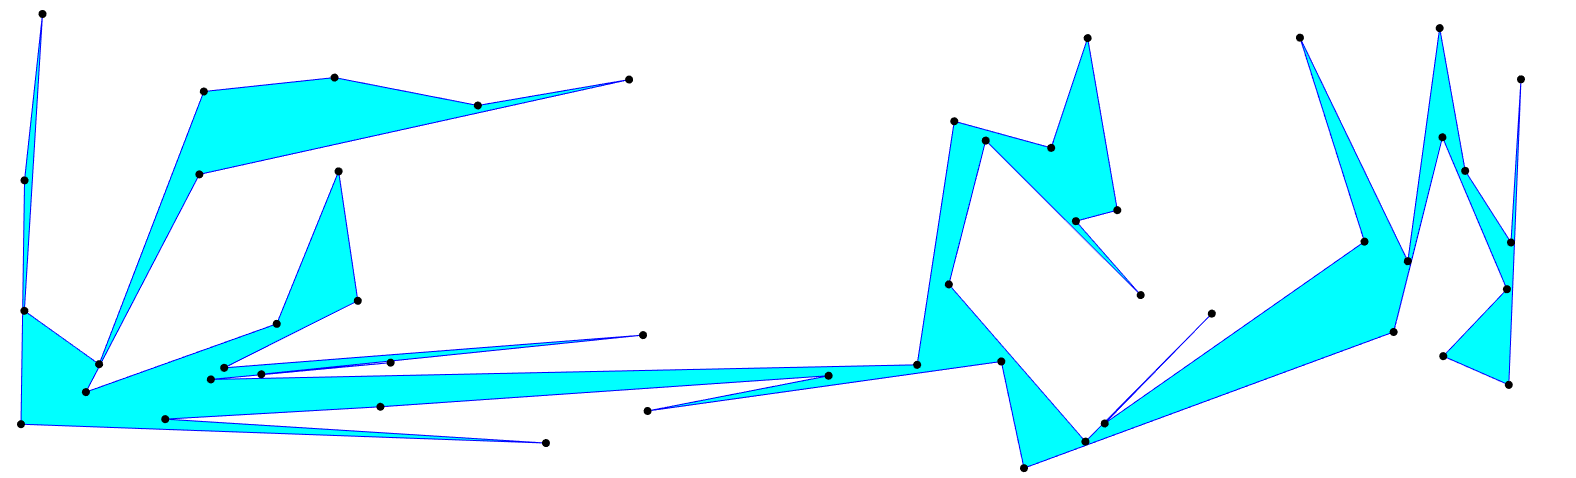
\includegraphics[width=0.99\textwidth]{fig6e.png}
				\caption{}
				\label{fig6e}
			\end{subfigure}
			
			\begin{subfigure}{0.85\linewidth}
				\centering
				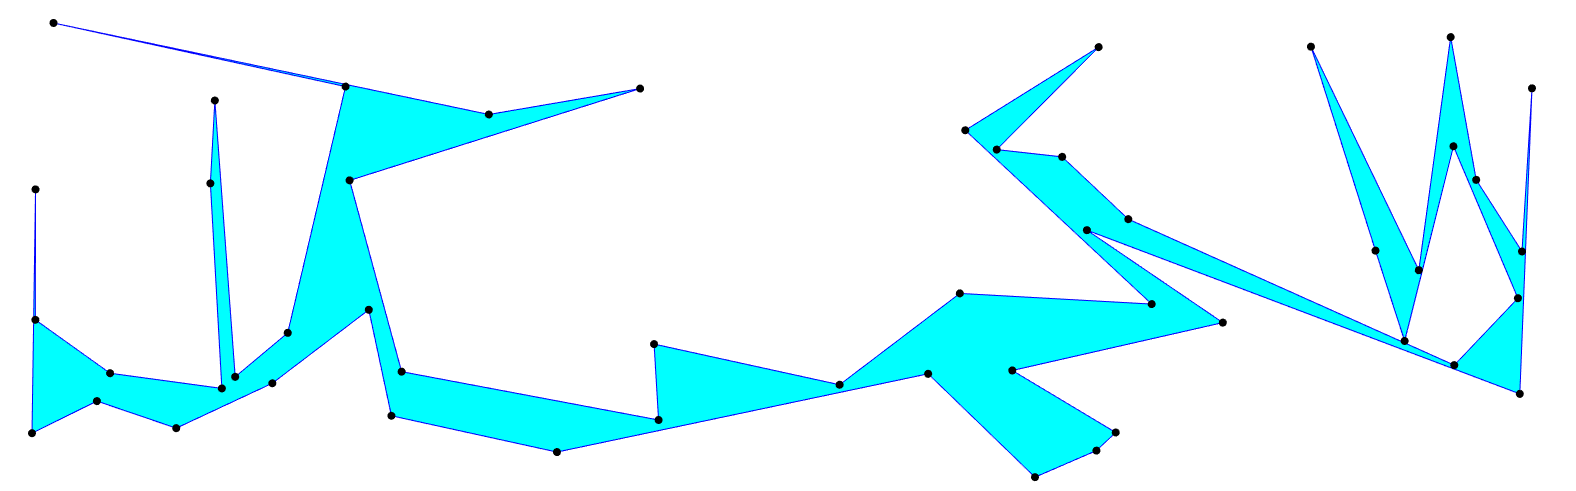
\includegraphics[width=0.99\textwidth]{fig6f.png}
				\caption{}
				\label{fig6f}
			\end{subfigure}
			
			\caption
			{
				Polygonalization of 5{\textunderscore}square.txt.
				(a) MAP{\textunderscore}DAC2
				(b) MAP{\textunderscore}DAC
				(c) MAP{\textunderscore}Greedy
				(d) MAP{\textunderscore}RAND
				(e) MAP{\textunderscore}RS
				(f) MAP{\textunderscore}DAC2{\textunderscore}P
			}
			\label{fig6}
		\end{figure}
		
		\begin{table*}[htbp]
			\begin{center}
				\caption{Comparison of results obtained from MAP{\textunderscore}DAC2, MAP{\textunderscore}DAC, MAP{\textunderscore}Greedy, MAP{\textunderscore}RAND, MAP{\textunderscore}RS.}
				\begin{tabular}{|c|c|c|c|c|c|c|}
					\hline
					File name & Number of points & \textbf{MAP{\textunderscore}DAC2} & MAP{\textunderscore}DAC & MAP{\textunderscore}Greedy & MAP{\textunderscore}RAND & \textbf{MAP{\textunderscore}RS} \\
					\hline
					0{\textunderscore}circle.txt & 50 & 1546.95 & 2205.22 & 2163.97 & 1421.74 & \textbf{1337.32} \\
					0{\textunderscore}grid.txt & 225 & \textbf{5073.6} & 7552.84 & 5893.04 & 6450.58 & 5136.01 \\
					0{\textunderscore}square.txt & 20 & 1649.18 & 2569.88 & 1783.53 & 1347.51 & \textbf{1275.03} \\
					\hline
					1{\textunderscore}circle.txt & 100 & 1407.81 & 2478.42 & 1613.12 & 1285.63 & \textbf{1245.65} \\
					1{\textunderscore}grid.txt & 324 & \textbf{7509.8} & 10717.5 & 9285.85 & 9478.32 & 7556.45 \\
					1{\textunderscore}square.txt & 70 & 2029.32 & 2206.15 & 2844.91 & 1834.54 & \textbf{1613.95} \\
					\hline
					2{\textunderscore}circle.txt & 150 & 1459.24 & 2173.04 & 2132.49 & 1606.34 & \textbf{1402.67} \\
					2{\textunderscore}grid.txt & 441 & \textbf{10196.1} & 14775.8 & 12771.9 & 12862.2 & 10229.6 \\
					2{\textunderscore}square.txt & 220 & 2022.32 & 3182.49 & 2937.25* & 2242.83 & \textbf{1869.77} \\
					\hline
					3{\textunderscore}circle.txt & 200 & 1565.39 & 2702.54 & 1597.23 & 1674.86 & \textbf{1398.37} \\
					3{\textunderscore}grid.txt & 576 & \textbf{13397.4} & 19157.1 & 18039.6 & 16774.6 & 13640.4 \\
					3{\textunderscore}square.txt & 470 & \textbf{1851.76} & 2916.31 & 2669.09 & 2294.82 & 1903.7 \\
					\hline
					4{\textunderscore}circle.txt & 250 & 1534.87 & 2405.29 & 1873.09 & 1704.48 & \textbf{1466.64} \\
					4{\textunderscore}grid.txt & 729 & \textbf{16209.4} & 22362.3 & 20766.8* & 21420.7 & 17387.4 \\
					4{\textunderscore}square.txt & 820 & \textbf{1881.42} & 2910.44 & 2708.03 & 2452.73 & 2018.38 \\
					\hline
					5{\textunderscore}circle.txt & 300 & 1533.45 & 2192.7 & 2027.85 & 1805.44 & \textbf{1479.12} \\
					5{\textunderscore}grid.txt & 900 & \textbf{19876} & 28519.2 & 26701.5 & 26726.3 & 21612.8 \\
					5{\textunderscore}square.txt & 50 & 589.507 & 797.318 & 681.784 & 594.001 & \textbf{497.325} \\
					\hline
					6{\textunderscore}circle.txt & 350 & \textbf{1441.19} & 2430.5 & 1901.1 & 1792.82 & 1475.15 \\
					6{\textunderscore}grid.txt & 330 & \textbf{6667.67} & 10850.5 & 9933.22* & 8969.63 & 7247.62 \\
					6{\textunderscore}square.txt & 140 & 560.736 & 875.54 & 680.984 & 597.184 & \textbf{530.764} \\
					\hline
					7{\textunderscore}circle.txt & 400 & \textbf{1397.47} & 2552.57 & 1923.42 & 1809.85 & 1492.82 \\
					7{\textunderscore}grid.txt & 360 & \textbf{7818.05} & 12676.4 & 10598.4* & 9783.51 & 8104.49 \\
					7{\textunderscore}square.txt & 290 & 564.116 & 933.543 & 741.509 & 675.447 & \textbf{561.196} \\
					\hline
					8{\textunderscore}circle.txt & 450 & \textbf{1485.48} & 2288.47 & 1966.1 & 1695.7 & 1515.07 \\
					8{\textunderscore}grid.txt & 390 & \textbf{7870.21} & 13452.7 & 11478.4 & 10362.4 & 8182.76 \\
					8{\textunderscore}square.txt & 500 & \textbf{548.995} & 973.862 & 772.515 & 701.326 & 573.593 \\
					\hline
					9{\textunderscore}circle.txt & 500 & \textbf{1536.36} & 2544.76 & 2084.82 & 1819.55 & 1591.75 \\
					9{\textunderscore}grid.txt & 420 & 9318.83 & 13578.1 & 12283.1 & 11080.6 & \textbf{8967.92} \\
					9{\textunderscore}square.txt & 770 & \textbf{561.227} & 945.21 & 826.275* & 718.896 & 567.384 \\ 
					\hline
				\end{tabular}
				\label{table1}
			\end{center}
		\end{table*}
	
		We also ran postprocessing on output from all algorithms on all point sets (Fig. \ref{fig6} (f)).
%		Table \ref{table2} shows areas of polygons after postprocessing in percentages relative to the area before postprocessing.
		We emphasize that postprocessing allows decreasing the area of solutions up to 10-25\%.
		Table \ref{table3} shows results after postprocessing.
		The result is improved by 18.7\% on average.
		MAP{\textunderscore}DAC2{\textunderscore}P outputs the best result in 17 cases, MAP{\textunderscore}RS{\textunderscore}P in 11 cases, and MAP{\textunderscore}RAND{\textunderscore}P in 2 cases.
		We apply postprocessing only to the best output of MAP{\textunderscore}RS and MAP{\textunderscore}RAND.
		It is expected to get even better results if postprocessing is applied after every trial of randomized algorithms.
		
\iffalse
		\begin{table*}[htbp]
			\begin{center}
				\caption{Area of polygons after postprocessing relative to Table 1 (\%).}
				\begin{tabular}{|c|c|c|c|c|c|}
					\hline
					File name & MAP{\textunderscore}DAC2{\textunderscore}P & MAP{\textunderscore}DAC{\textunderscore}P & MAP{\textunderscore}Greedy{\textunderscore}P & MAP{\textunderscore}RAND{\textunderscore}P & MAP{\textunderscore}RS{\textunderscore}P \\
					\hline
					0{\textunderscore}circle.txt & 83.2882 & 68.8231 & 74.8971 & 95.2749 & 86.6654 \\
					0{\textunderscore}grid.txt & 78.4822 & 60.7262 & 93.39 & 83.7179 & 85.1955 \\
					0{\textunderscore}square.txt & 86.2036 & 56.9215 & 91.4348 & 100 & 98.5454 \\
					\hline
					1{\textunderscore}circle.txt & 75.0139 & 53.6432 & 92.613 & 74.8542 & 92.1643 \\
					1{\textunderscore}grid.txt & 77.4988 & 60.4907 & 89.2939 & 79.3326 & 75.3776 \\
					1{\textunderscore}square.txt & 84.4191 & 81.2336 & 88.9499 & 82.773 & 95.9746 \\
					\hline
					2{\textunderscore}circle.txt & 84.6908 & 68.3225 & 82.913 & 83.7697 & 82.2322 \\
					2{\textunderscore}grid.txt & 76.7843 & 59.1727 & 91.3193 & 81.1598 & 83.3493 \\
					2{\textunderscore}square.txt & 77.272 & 60.4619 & 89.8424 & 71.8307 & 91.8665 \\
					\hline
					3{\textunderscore}circle.txt & 82.1769 & 55.8258 & 94.2239 & 77.7306 & 85.2177 \\
					3{\textunderscore}grid.txt & 74.7865 & 55.3249 & 88.3407 & 80.2147 & 83.075 \\
					3{\textunderscore}square.txt & 79.7649 & 59.1584 & 85.9197 & 74.7312 & 87.1332 \\
					\hline
					4{\textunderscore}circle.txt & 77.9657 & 62.6643 & 92.1431 & 82.6544 & 83.4875 \\
					4{\textunderscore}grid.txt & 81.1176 & 62.3924 & 83.0463 & 76.909 & 81.0698 \\
					4{\textunderscore}square.txt & 79.6647 & 59.2644 & 83.1866 & 76.7587 & 77.6908 \\
					\hline
					5{\textunderscore}circle.txt & 81.8064 & 63.7366 & 84.6136 & 84.7903 & 78.679 \\
					5{\textunderscore}grid.txt & 78.9024 & 59.4176 & 85.437 & 80.5203 & 79.2287 \\
					5{\textunderscore}square.txt & 82.5412 & 70.5668 & 93.033 & 85.7604 & 82.9386 \\
					\hline
					6{\textunderscore}circle.txt & 85.8389 & 60.589 & 85.0262 & 77.9972 & 83.1042 \\
					6{\textunderscore}grid.txt & 77.2097 & 66.6462 & 87.6776 & 78.2857 & 85.3425 \\
					6{\textunderscore}square.txt & 83.7059 & 64.268 & 78.2077 & 85.5597 & 86.3094 \\
					\hline
					7{\textunderscore}circle.txt & 80.6722 & 62.6201 & 82.9018 & 77.7518 & 80.1766 \\
					7{\textunderscore}grid.txt & 76.3475 & 65.5676 & 83.5795 & 80.737 & 81.5681 \\
					7{\textunderscore}square.txt & 82.0708 & 57.3291 & 86.3043 & 83.8413 & 83.6514 \\
					\hline
					8{\textunderscore}circle.txt & 81.367 & 63.3459 & 79.5047 & 72.7502 & 79.4567 \\
					8{\textunderscore}grid.txt & 75.0734 & 66.7353 & 86.8286 & 77.9401 & 80.2878 \\
					8{\textunderscore}square.txt & 80.2742 & 56.8465 & 82.3947 & 80.5178 & 85.0199 \\
					\hline
					9{\textunderscore}circle.txt & 77.5403 & 57.7584 & 89.2339 & 74.1333 & 82.8734 \\
					9{\textunderscore}grid.txt & 81.2925 & 64.3985 & 80.572 & 79.5746 & 81.9839 \\
					9{\textunderscore}square.txt & 77.0793 & 61.8968 & 81.2972 & 74.8826 & 82.044 \\
					\hline
				\end{tabular}
				\label{table2}
			\end{center}
		\end{table*}
\fi
		
		\begin{table*}[htbp]
			\begin{center}
				\caption{Postprocessing. Comparison of results obtained from MAP{\textunderscore}DAC2{\textunderscore}P, MAP{\textunderscore}DAC{\textunderscore}P, MAP{\textunderscore}Greedy{\textunderscore}P, MAP{\textunderscore}RAND{\textunderscore}P, MAP{\textunderscore}RS{\textunderscore}P.}
				\begin{tabular}{|c|c|c|c|c|c|c|c|}
					\hline
					File name & DAC2{\textunderscore}P & DAC{\textunderscore}P & Greedy{\textunderscore}P & RAND{\textunderscore}P & RS{\textunderscore}P & Result before postprocessing & Result after postprocessing \\
					\hline
					0{\textunderscore}circle.txt & 1288.43 & 1517.7 & 1620.75 & 1354.56 & \textbf{1158.99} & 1337.32 & \textbf{1158.99} \\
					0{\textunderscore}grid.txt & \textbf{3981.88} & 4586.55 & 5503.51 & 5400.29 & 4375.65 & 5073.6 & \textbf{3981.88} \\
					0{\textunderscore}square.txt & 1421.65 & 1462.81 & 1630.76 & 1347.51 & \textbf{1256.49} & 1275.03 & \textbf{1256.49} \\
					\hline
					1{\textunderscore}circle.txt & 1056.05 & 1329.5 & 1493.96 & \textbf{962.349} & 1148.04 & 1245.65 & \textbf{962.349} \\
					1{\textunderscore}grid.txt & 5820 & 6483.09 & 8291.7 & 7519.4 & \textbf{5695.87} & 7509.8 & \textbf{5695.87} \\
					1{\textunderscore}square.txt & 1713.14 & 1792.14 & 2530.54 & \textbf{1518.5} & 1548.98 & 1613.95 & \textbf{1518.5} \\
					\hline
					2{\textunderscore}circle.txt & 1235.84 & 1484.68 & 1768.12 & 1345.62 & \textbf{1153.44} & 1402.67 & \textbf{1153.44} \\
					2{\textunderscore}grid.txt & \textbf{7829.01} & 8743.24 & 11663.3 & 10438.9 & 8526.33 & 10196.1 & \textbf{7829.01} \\
					2{\textunderscore}square.txt & \textbf{1562.69} & 1924.19 & 2638.89 & 1611.04 & 1717.69 & 1869.77 & \textbf{1562.69} \\
					\hline
					3{\textunderscore}circle.txt & 1286.39 & 1508.71 & 1504.97 & 1301.88 & \textbf{1191.66} & 1398.37 & \textbf{1191.66} \\
					3{\textunderscore}grid.txt & \textbf{10019.5} & 10598.7 & 15936.3 & 13455.7 & 11331.8 & 13397.4 & \textbf{10019.5} \\
					3{\textunderscore}square.txt & \textbf{1477.05} & 1725.24 & 2293.27 & 1714.95 & 1658.75 & 1851.76 & \textbf{1477.05} \\
					\hline
					4{\textunderscore}circle.txt & \textbf{1196.67} & 1507.26 & 1725.93 & 1408.83 & 1224.46 & 1466.64 & \textbf{1196.67} \\
					4{\textunderscore}grid.txt & \textbf{13148.7} & 13952.4 & 17246.1 & 16474.5 & 14095.9 & 16209.4 & \textbf{13148.7} \\
					4{\textunderscore}square.txt & \textbf{1498.83} & 1724.86 & 2252.72 & 1882.68 & 1568.09 & 1881.42 & \textbf{1498.83} \\
					\hline
					5{\textunderscore}circle.txt & 1254.46 & 1397.55 & 1715.84 & 1530.84 & \textbf{1163.76} & 1479.12 & \textbf{1163.76} \\
					5{\textunderscore}grid.txt & \textbf{15682.7} & 16945.4 & 22812.9 & 21520.1 & 17123.5 & 19876 & \textbf{15682.7} \\
					5{\textunderscore}square.txt & 486.586 & 562.642 & 634.284 & 509.418 & \textbf{412.474} & 497.325 & \textbf{412.474} \\
					\hline
					6{\textunderscore}circle.txt & 1237.1 & 1472.61 & 1616.43 & 1398.35 & \textbf{1225.92} & 1441.19 & \textbf{1225.92} \\
					6{\textunderscore}grid.txt & \textbf{5148.09} & 7231.47 & 8709.21 & 7021.94 & 6185.3 & 6667.67 & \textbf{5148.09} \\
					6{\textunderscore}square.txt & 469.369 & 562.691 & 532.582 & 510.949 & \textbf{458.1} & 530.764 & \textbf{458.1} \\
					\hline
					7{\textunderscore}circle.txt & \textbf{1127.37} & 1598.42 & 1594.55 & 1407.19 & 1196.89 & 1397.47 & \textbf{1127.37} \\
					7{\textunderscore}grid.txt & \textbf{5968.88} & 8311.64 & 8858.07 & 7898.91 & 6610.68 & 7818.05 & \textbf{5968.88} \\
					7{\textunderscore}square.txt & \textbf{462.974} & 535.192 & 639.955 & 566.304 & 469.448 & 561.196 & \textbf{462.974} \\
					\hline
					8{\textunderscore}circle.txt & 1208.69 & 1449.65 & 1563.14 & 1233.62 & \textbf{1203.83} & 1485.48 & \textbf{1203.83} \\
					8{\textunderscore}grid.txt & \textbf{5908.43} & 8977.68 & 9966.53 & 8076.5 & 6569.76 & 7870.21 & \textbf{5908.43} \\
					8{\textunderscore}square.txt & \textbf{440.701} & 553.607 & 636.511 & 564.692 & 487.669 & 548.995 & \textbf{440.701} \\
					\hline
					9{\textunderscore}circle.txt & \textbf{1191.3} & 1469.81 & 1860.37 & 1348.89 & 1319.14 & 1536.36 & \textbf{1191.3} \\
					9{\textunderscore}grid.txt & 7575.51 & 8744.08 & 9896.72 & 8817.38 & \textbf{7352.25} & 8967.92 & \textbf{7352.25} \\
					9{\textunderscore}square.txt & \textbf{432.59} & 585.055 & 671.739 & 538.328 & 465.505 & 561.227 & \textbf{432.59} \\
					\hline
				\end{tabular}
				\label{table3}
			\end{center}
		\end{table*}
	
	\section{Conclusion}
	\label{S5}
		In this paper, we present modification (MAP{\textunderscore}DAC2) to the Divide and Conquer based algorithm for constructing an approximate solution of the MAP problem.
		The algorithm computes slightly more cases compared to the unmodified version but shows significant improvement in the polygon area.
		The complexity of the algorithm is $O(n^{2}log(n))$ using $O(n)$ memory.
		We also propose the algorithm for postprocessing output of other algorithms that improves local optimality via local rearrangements point by point.
		The complexity of postprocessing is $O(n^{2})$ using $O(n)$ memory.
	
		We conduct experimental study to compare existing algorithms.
		MAP{\textunderscore}DAC2 turns out to be competitive in terms of polygonalization area while working much faster than the best of existing algorithms.
		We also compare results before and after postprocessing.
		Postprocessing improved best polygonalizations by 18\% on average which is an outstanding result.
	
		During the research of existing and new MAP algorithms, we considered 3 tactics -- producing new polygonalization, postprocessing of polygonalization, and constructing new better polygonalizations via combining other polygonalizations.
		Producing new polygonalization is relatively well studied in the literature.
		We propose the first MAP postprocessing technique in this paper.
		Polygon combining is left for future research.
		We believe that all 3 tactics deserve further investigation.
	
%	\clearpage
	
	\begin{thebibliography}{00}
		\bibitem{link1} Worboys, M., \& Duckham, M. (2006). Monitoring qualitative spatiotemporal change for geosensor networks. International Journal of Geographical Information Science, 20(10), 1087–1108.
		\bibitem{link2} Galton, A. (2005). Dynamic Collectives and Their Collective Dynamics. In Spatial Information Theory (pp. 300–315). Springer Berlin Heidelberg.
		\bibitem{link3} Miller, H. J., \& Han, J. (Eds.). (2009). Geographic Data Mining and Knowledge Discovery. CRC Press.
		\bibitem{link4} Galton, A., \& Duckham, M. (2006). What Is the Region Occupied by a Set of Points? In Geographic Information Science (pp. 81–98). Springer Berlin Heidelberg.
		\bibitem{link5} Fekete, S. P. (2000). On Simple Polygonalizations with Optimal Area. Discrete \& Computational Geometry, 23(1), 73–110.
		\bibitem{link6} Kumar, S. (1996). Surface Triangulation: A Survey.
		\bibitem{link7} Eppstein, D., Overmars, M., Rote, G., \& Woeginger, G. (1992). Finding minimum areak-gons. Discrete \& Computational Geometry, 7(1), 45–58.
		\bibitem{link8} V. Tereshchenko, V. Muravitskiy, Constructing a simple polygonalizations. Journal of World Academy of Science, Engineering and Technology (77), pp. 668-671, 2011.
		\bibitem{link9} Fekete, S., Friedrichs, S., Hemmer, M., Papenberg, M., Schmidt, A., \& Troegel, J. (2015). Area- and Boundary-Optimal Polygonalization of Planar Point Sets. EuroCG 2015.
		\bibitem{link10} Fekete, S., Haas, A., Keldenich, P., Perk, M., \& Schmidt, A. (2020). Computing Area-Optimal Simple Polygonalizations.
		\bibitem{link11} Peethambaran, J., Parakkat, A. D., \& Muthuganapathy, R. (2016). An Empirical Study on Randomized Optimal Area Polygonization of Planar Point Sets. ACM Journal of Experimental Algorithmics, 21, 1–24.
		\bibitem{link12} Taranilla, María Teresa and Gagliardi, Edilma Olinda and Hernández Peñalver, Gregorio (2011). Approaching minimum area polygonization. XVII Congreso Argentino de Ciencias de la Computación 2011, Argentina, pp. 161-170.
		\bibitem{link13} Osiponok, M., \& Tereshchenko, V. (2019, December). The “Divide and Conquer” technique to solve the Minimum Area Polygonalization problem. 2019 IEEE International Conference on Advanced Trends in Information Theory (ATIT). 2019 IEEE International Conference on Advanced Trends in Information Theory (ATIT).
		\bibitem{link14} B.Joe, R.B. Simpson, Corrections to lee's visibility polygon algorithm. BIT Numerical Mathematics 27(4), pp. 458-473, 1987.
	\end{thebibliography}

\end{document}

















